\documentclass[a4paper,12pt, oneside]{article}

\usepackage[utf8]{inputenc}
\usepackage[french]{babel}
\usepackage{url}  % Pour utiliser \url{...} dans les références
\usepackage{graphicx} % Pour insérer des images
\usepackage{setspace} % Pour gérer l'interligne
\usepackage{xcolor}
\usepackage{tcolorbox}
\usepackage[T1]{fontenc} 
\usepackage{booktabs}
\usepackage{newtxtext} % Texte en Times New Roman
\usepackage{newtxmath} % Symboles mathématiques compatibles Times
\usepackage{array} % Vertical Alignement Table
\usepackage[margin=1.75cm, bottom=2.5cm]{geometry} 
%packages pour ajouter le code python 
\usepackage{listings}
\usepackage{multicol}
\definecolor{codebackground}{rgb}{0.95, 0.95, 0.92}

% Set up the styling rules globally
\lstset{
    backgroundcolor=\color{codebackground}, % Background color
    basicstyle=\ttfamily\small,            % Font style (monospaced)
    breaklines=true,                       % Wrap long lines automatically
    frame=single,                          % Draw a clean thin box border
    rulecolor=\color{lightgray}            % Border line color
}
\usepackage{xcolor} % déjà présent, utile pour les couleurs dans le code
\usepackage{longtable}
\usepackage{fancyhdr}
\pagestyle{fancy}
\fancyhf{} % Completely clears the default top headers and bottom footers
% Put page number in the Center of the Footer for ALL pages
\fancyfoot[C]{\thepage} 
\renewcommand{\arraystretch}{1.2} 
\usepackage{titletoc}

% Redefine the List of Tables entry format
\titlecontents{table}
  [0pt]                                 % Left indent
  {\addvspace{0.5pc}}                   % Space above entry
  {Tableau \thecontentslabel : }                              
  {\hspace{0pt}}                        % Code for unnumbered entry
  {\titlerule*[0.5pc]{.}\quad page~\thecontentspage} % Filler dots + "page X"

% Note: Swapping the actual string data perfectly using native layout engines requires 
% the manual macro method above, because LaTeX natively passes the number *before* the caption.


% --- LIST OF FIGURES CUSTOMIZATION ---
\titlecontents{figure}
  [0pt]                                          % Left indent
  {\addvspace{0.5pc}}                            % Space above entry
  {Figure \thecontentslabel : }                      % FRONT NUMBERING: Prints "f1", "f2", etc.
  {\hspace{0pt}}                                 % Code for unnumbered entry
  {\titlerule*[0.5pc]{.}\quad page~\thecontentspage} % Filler dots + "page X"



\titlecontents{section}
  [1.5em]                               % Retrait à gauche
  {\addvspace{0.4pc}\bfseries}          % Espace au-dessus + Gras pour les sections
  {\contentslabel{1.5em}}               % Espace pour le numéro (ex: 1.)
  {\hspace{-1.5em}}                     % Si pas de numéro
  {\titlerule*[0.5pc]{.}\quad\thecontentspage}

% Pour les Subsections (Niveau 2)
\titlecontents{subsection}
  [3.8em]                               % Retrait plus grand pour décaler vers la droite
  {\addvspace{0.2pc}}                   % Espace léger au-dessus
  {\contentslabel{2.3em}}               % Espace pour le numéro (ex: 1.1.)
  {\hspace{-2.3em}}
  {\titlerule*[0.5pc]{.}\quad\thecontentspage}

% Pour les Subsubsections (Niveau 3)
\titlecontents{subsubsection}
  [6.8em]                               % Retrait encore plus grand
  {\addvspace{0.1pc}}
  {\contentslabel{3.0em}}               % Espace pour le numéro (ex: 1.1.1.)
  {\hspace{-3.0em}}
  {\titlerule*[0.5pc]{.}\quad\thecontentspage}




\definecolor{codegreen}{rgb}{0,0.6,0}
\definecolor{codegray}{rgb}{0.5,0.5,0.5}
\definecolor{codepurple}{rgb}{0.58,0,0.82}
\definecolor{backcolour}{rgb}{0.97,0.97,0.98}
\definecolor{codeblue}{rgb}{0,0,0.8}

\lstdefinestyle{pythonstyle}{
    backgroundcolor=\color{backcolour},
    commentstyle=\color{codegreen},
    keywordstyle=\color{codeblue}\bfseries,
    numberstyle=\tiny\color{codegray},
    stringstyle=\color{codepurple},
    basicstyle=\ttfamily\footnotesize,
    breakatwhitespace=false,
    breaklines=true,
    captionpos=b,
    keepspaces=true,
    numbers=left,
    numbersep=5pt,
    showspaces=false,
    showstringspaces=false,
    showtabs=false,
    tabsize=4,
    frame=single,
    rulecolor=\color{codegray},
    language=Python
}

\lstset{style=pythonstyle}





% Remove the horizontal lines
\renewcommand{\headrulewidth}{0pt}
\renewcommand{\footrulewidth}{0pt}

% Force chapter opening pages to also use this exact same style
\fancypagestyle{plain}{
  \fancyhf{}
  \fancyfoot[C]{\thepage}
}

% 1. Change the title from "Contents" to your preference (e.g., "Table des matières")
\renewcommand{\contentsname}{
\begin{center}
\LARGE
SOMMAIRE
\end{center}
}

\addto\captionsfrench{
  % Pour le Sommaire
  \renewcommand{\contentsname}{
    \begin{center}
    \LARGE
    SOMMAIRE
    \end{center}
  }
  % Pour la Liste des Tableaux (LoT)
  \renewcommand{\listtablename}{
    \begin{center}
    \Large
    LISTE DES TABLEAUX
    \end{center}
  }
  % Pour la Liste des Figures (LoF)
  \renewcommand{\listfigurename}{
    \begin{center}
    \Large
    LISTE DES FIGURES
    \end{center}
  }
}

\definecolor{monbleu}{RGB}{0,0,255} % bleu pur RGB
\definecolor{bleuciel}{RGB}{90,170,210} % bleu ciel


% 2. Limit ToC depth to Level-2 headings (\subsection)
%\setcounter{tocdepth}{2}
%\makeatletter
%\let\oldcontentsline\contentsline
%\renewcommand{\contentsline}[4]{%
  % This strips out the page number variable (#3) from compiling inside the ToC rows
 % \oldcontentsline{#1}{#2}{}{#4}%
%}
%\renewcommand{\@dotsep}{10000} % Enlève les pointillés sur la TOC
%\makeatother



% \renewcommand{\chaptername}{Chapitre} 
\usepackage{float}

\begin{document}

\begin{titlepage}
\centering

\vspace*{0.5cm}


\includegraphics[width=5cm]{logo_insi.png}

\vspace{0.3cm}


\noindent\rule{0.7\textwidth}{0.4pt}

\vspace{0.8cm}

\textbf{\large INSTITUT NATIONAL SUPERIEUR D'INFORMATIQUE}

\vspace{0.8cm}

\textbf{Mémoire de projet en vue de la validation de la Licence 2}

\vspace{0.6cm}

Domaine : Sciences et Technologie

Mention : Informatique

Parcours : Intelligence Artificielle et Data Science

\vspace{0.8cm}

\textbf{Par :} ANDRIAMIHAJAMANANA Anjara \\

\vspace{1cm}

\textbf{\Large Système Intelligent d'Analyse des Productions Halieutiques}

\vspace{0.8cm}

Soutenu le 07 Septembre 2026, devant la commission d'examen composée de :

\vspace{0.5cm}

Président du Jury :
Docteur RAKOTOMANANA René

\vspace{0.5cm}

Examinateur :
Docteur RANDRIAMAMONJY Liantsoa Joharinirina

\vspace{0.5cm}

Encadreur :
Docteur ANDRIAMANJAKA Ramasondrano

\vfill

\textbf{Année Universitaire : 2025-2026}

\end{titlepage}


\thispagestyle{empty}
\vspace*{\fill}
\newpage


\pagenumbering{roman}
\begin{center}
\LARGE{REMERCIEMENTS}
\end{center}

Avant toute chose, je tiens à exprimer ma profonde gratitude envers Dieu, pour la force, la santé et la persévérance qu'Il m'a accordées tout au long de la réalisation de ce travail.\\

Je tiens ensuite à exprimer ma sincère reconnaissance au Dr Ingénieur RAMASONDRANO Andriamanjaka, Directeur de l'école, qui a également assuré l'encadrement de ce mémoire. Malgré ses nombreuses responsabilités à la tête de l'établissement, il a su m'accorder de son temps précieux, me prodiguer des conseils avisés et m'accompagner avec rigueur et bienveillance tout au long de ce mémoire.\\

Mes remerciements vont aussi à l'ensemble des enseignants, pour la qualité de l'enseignement dispensé , ainsi qu'aux membres du jury, pour avoir accepté d'évaluer ce travail et pour l'intérêt qu'ils y ont porté.\\

Enfin, je ne saurais oublier ma famille et mes proches, dont le soutien indéfectible, a été un pilier essentiel. Je remercie également mes amis pour leur présence et leur soutien tout au long de ce mémoire.\\

À toutes celles et à tous ceux qui, de près ou de loin, ont contribué à la réalisation de ce travail, j'adresse mes sincères remerciements.
\vspace*{\fill}
\newpage
\begin{spacing}{1.5}
\begin{center}
\LARGE{RÉSUMÉ}
\end{center}

La rizipisciculture, qui associe l'élevage de tilapia à la culture du riz, présente un potentiel économique, social et environnemental important à Madagascar, mais son développement reste freiné par l'absence d'outils fiables de surveillance et d'anticipation de la qualité de l'eau, exposant les exploitations à des risques de dégradation souvent détectés trop tard. Ce mémoire répond ainsi à la problématique suivante : comment analyser la qualité de l'eau et les conditions environnementales d'une parcelle de rizipisciculture afin de protéger, anticiper et optimiser la production de tilapia ? L'objectif est de concevoir un système intelligent composé de trois modules complémentaires.\\

Pour atteindre cet objectif, le premier module estime la densité de tilapia atteignable à partir des caractéristiques du sol, à l'aide de modèles de régression tels que la Régression Linéaire, le SVR, l'Arbre de Décision, la Random Forest et XGBoost, optimisés par GridSearch. Le deuxième module classe l'état actuel de la qualité de l'eau en bonne ou mauvaise qualité pour le tilapia, selon la même démarche appliquée à des modèles de classification. Le troisième module anticipe l'évolution de la qualité de l'eau à l'horizon d'une heure, en combinant une décomposition STL et un réseau de neurones récurrent LSTM, afin de déclencher une alerte préventive en cas de dégradation anticipée.\\

Les résultats montrent que les modèles à base d'ensembles d'arbres, en particulier la Random Forest et XGBoost, offrent les meilleures performances pour l'estimation de la densité et la classification de la qualité de l'eau, avec un rappel supérieur à 0,92 pour ce dernier module. L'approche STL-LSTM atteint un pouvoir explicatif élevé pour l'ensemble des paramètres physico-chimiques prédits. Une interface de démonstration a enfin été développée pour illustrer l'usage concret du système, constituant une première contribution vers un outil d'aide à la décision destiné aux rizipisciculteurs malgaches.

\vspace{0.5cm}
\textbf{Mots-clés :} rizipisciculture, tilapia, qualité de l'eau, machine learning, GridSearch, STL, LSTM.
\end{spacing}

\vspace*{\fill}
\newpage
\begin{spacing}{1.5}
\begin{center}
\LARGE{ABSTRACT}
\end{center}
Rice-fish farming, which combines tilapia rearing with rice cultivation, holds significant economic, social, and environmental potential in Madagascar, but its development is hindered by the lack of reliable tools to monitor and anticipate water quality, exposing farms to degradation risks that are often detected too late. This thesis addresses the following question: how can water quality and environmental conditions of a rice-fish farming plot be analyzed to protect, anticipate, and optimize tilapia production? The objective is to design an intelligent system made up of three complementary modules.

To achieve this, the first module estimates achievable tilapia density from soil characteristics, using regression models such as Linear Regression, SVR, Decision Tree, Random Forest, and XGBoost, optimized through GridSearch. The second module classifies current water quality as good or poor for tilapia, following the same approach applied to classification models. The third module anticipates water quality evolution one hour ahead, combining STL decomposition with an LSTM recurrent neural network, in order to trigger a preventive alert in case of anticipated degradation.

The results show that ensemble tree-based models, particularly Random Forest and XGBoost, achieve the best performance for density estimation and water quality classification, reaching a recall above 0.92 for the latter module. The STL-LSTM approach achieves strong explanatory power across all predicted physico-chemical parameters. A demonstration interface was finally developed to illustrate the practical use of the system, forming an initial contribution toward a decision-support tool for Malagasy rice-fish farmers.

\vspace{0.5cm}
\textbf{Keywords:} rice-fish farming, tilapia, water quality, machine learning, GridSearch, STL, LSTM.
\end{spacing}

\vspace*{\fill}
\newpage

\tableofcontents
\vspace*{\fill}
\newpage

\begin{center}
\Large LISTE DES ABREVIATIONS
\end{center}

\begin{longtable}{|p{3.5cm}|p{13cm}|}
\hline
\textbf{Sigle} & \textbf{Signification} \\
\hline
APDRA & Association Pisciculture et Développement Rural en Afrique \\
\hline
ARSB & Administration Réseaux et Systèmes et Bases de données \\
\hline
CV & Cross-Validation (validation croisée) \\
\hline
DO & Dissolved Oxygen (oxygène dissous) \\
\hline
FAO & Food and Agriculture Organization (Organisation des Nations Unies pour l'alimentation et l'agriculture) \\
\hline
FOFIFA & Foibem-pirenena momba ny Fikarohana ampiharina amin'ny Fampandrosoana ny eny Ambanivohitra\\
\hline
GL & Génie Logiciel \\
\hline
I2AD & Intelligence Artificielle, Analyse de Données et Automatisation \\
\hline
IAD & Intelligence Artificielle et Data Science \\
\hline
IC & Infrastructures et Cybersécurités \\
\hline
IISD & Institut International du Développement Durable \\
\hline
INSI & Institut National Supérieur d'Informatique \\
\hline
IoT & Internet of Things (Internet des objets) \\
\hline
IPNA & Infrastructure Publique Numérique Agricole \\
\hline
LMD & Licence-Master-Doctorat \\
\hline
LSTM & Long Short-Term Memory \\
\hline
MAE & Mean Absolute Error \\
\hline
MAPE & Mean Absolute Percentage Error \\
\hline
MINAE & Ministère de l'Agriculture et de la Souveraineté Alimentaire (Madagascar) \\
\hline
MSI & Management des Systèmes d'Information \\
\hline
NTU & Nephelometric Turbidity Unit \\
\hline
PADM & Projet d'Aquaculture Durable à Madagascar \\
\hline
PIB & Produit Intérieur Brut \\
\hline
RMSE & Root Mean Squared Error \\
\hline
RNN & Recurrent Neural Network \\
\hline
SVC & Support Vector Classification \\
\hline
SVM & Support Vector Machine \\
\hline
SVR & Support Vector Regression \\
\hline
STL & Seasonal-Trend decomposition using Loess \\
\hline
\end{longtable}

\vspace*{\fill}
\newpage

\begin{center}
\LARGE GLOSSAIRE
\end{center}

\begin{longtable}{@{}p{4cm}p{13cm}@{}}
\textbf{Terme} & \textbf{Définition} \\
\midrule

Accuracy & Proportion globale de prédictions correctes d'un modèle de classification, sur l'ensemble des observations \cite{scikitlearn}. \\[24pt]
Disparition du gradient (vanishing gradient) & Phénomène par lequel le gradient utilisé pour ajuster les poids d'un réseau de neurones récurrent devient de plus en plus faible à mesure qu'il est rétropropagé sur une séquence longue, empêchant le modèle de retenir une information sur le long terme \cite{hochreiter1997}. \\[24pt]
Downsampling & Technique de rééquilibrage des classes consistant à réduire aléatoirement le nombre d'observations de la classe majoritaire pour l'égaliser à celui de la classe minoritaire \cite{imblearndoc}. \\[24pt]
Élagage (pruning) & Technique consistant à supprimer, après la construction d'un arbre de décision, les branches apportant peu de gain prédictif, afin de réduire sa complexité et de limiter le surapprentissage \cite{scikitlearn}. \\[24pt]
Encodage ordinal & Transformation d'une variable catégorielle en valeurs numériques entières croissantes, adaptée lorsque ses modalités possèdent un ordre naturel \cite{scikitlearn}. \\[24pt]
Encodage one-hot & Transformation d'une variable catégorielle en plusieurs colonnes binaires distinctes, adaptée lorsque ses modalités n'ont pas de relation d'ordre entre elles \cite{scikitlearn}. \\[24pt]
Entropie & Mesure du désordre ou de l'incertitude des classes présentes dans un nœud d'un arbre de décision, utilisée comme critère alternatif à l'impureté de Gini pour évaluer la qualité d'un découpage \cite{scikitlearn}. \\[24pt]
F1-score & Métrique combinant la Precision et le Recall en une seule valeur, utile pour comparer des modèles de classification de façon synthétique \cite{scikitlearn}. \\[24pt]
Feature Engineering & Ensemble des techniques de transformation, de sélection ou de création de variables à partir des données brutes, afin d'améliorer la capacité d'un modèle à apprendre une tâche donnée \cite{scikitlearn}. \\[24pt]
Fenêtre glissante (sliding window) & Méthode de structuration d'une série temporelle consistant à utiliser un nombre fixe d'observations passées consécutives comme variables d'entrée pour prédire l'observation suivante \cite{fpp3}. \\[24pt]
Impureté de Gini & Mesure de la probabilité de mal classer une observation tirée au hasard selon la distribution des classes d'un nœud, utilisée comme critère de découpage dans un arbre de décision \cite{scikitlearn}. \\[24pt]
GridSearch & Méthode d'optimisation testant systématiquement toutes les combinaisons d'une grille d'hyperparamètres candidats, généralement combinée à une validation croisée \cite{scikitlearn}. \\[24pt]
Hyperparamètre & Paramètre d'un modèle fixé avant l'entraînement, par opposition aux paramètres appris automatiquement pendant l'entraînement \cite{scikitlearn}. \\[24pt]
Kernel trick & Technique permettant à un modèle SVM de séparer des données non linéairement séparables, en calculant implicitement leur similarité dans un espace de dimension supérieure \cite{cortesvapnik1995}. \\[24pt]
LSTM (Long Short-Term Memory) & Architecture de réseau de neurones récurrent dotée d'un système de portes, capable de retenir des dépendances temporelles sur de longues séquences \cite{hochreiter1997}. \\[24pt]
MAE (Mean Absolute Error) & Métrique de régression correspondant à l'écart moyen absolu entre les valeurs prédites et les valeurs réelles \cite{scikitlearn}. \\[24pt]
MAPE (Mean Absolute Percentage Error) & Métrique de régression exprimant l'erreur moyenne en pourcentage de la valeur réelle \cite{fpp3}. \\[24pt]
Overfitting (surapprentissage) & Phénomène par lequel un modèle s'ajuste excessivement aux données d'entraînement, y compris à leur bruit, au détriment de sa capacité à généraliser sur de nouvelles données \cite{scikitlearn}. \\[24pt]
Precision & Parmi les observations prédites comme positives par un modèle de classification, proportion réellement positive \cite{scikitlearn}. \\[36pt]
Random Forest & Modèle d'ensemble combinant un grand nombre d'arbres de décision entraînés sur des échantillons et des sous-ensembles de variables différents, afin de réduire la variance et le surapprentissage \cite{breiman2001}. \\[24pt]
Recall (rappel) & Parmi les observations réellement positives, proportion correctement détectée par un modèle de classification \cite{scikitlearn}. \\[24pt]
RMSE (Root Mean Squared Error) & Métrique de régression pénalisant davantage les erreurs importantes, exprimée dans la même unité que la variable prédite \cite{fpp3}. \\[24pt]
Rizipisciculture & Pratique agroécologique associant l'élevage de poissons à la culture du riz sur une même parcelle inondée \cite{apdra2023}. \\[24pt]
$R^2$ (coefficient de détermination) & Métrique de régression indiquant la proportion de la variance de la variable cible expliquée par le modèle \cite{scikitlearn}. \\[24pt]
Standardisation (Z-score) & Technique de mise à l'échelle transformant une variable pour obtenir une moyenne nulle et un écart-type unitaire \cite{scikitlearn}. \\[24pt]
STL (Seasonal-Trend decomposition using Loess) & Méthode décomposant une série temporelle en une composante de tendance, une composante saisonnière et un résidu, à l'aide de la méthode de lissage Loess \cite{cleveland1990,statsmodelsdoc}. \\[36pt]
SVM (Support Vector Machine) & Modèle cherchant à séparer des données en classes à l'aide d'un hyperplan maximisant la marge entre les classes \cite{cortesvapnik1995}. \\[36pt]
Tilapia & Espèce de poisson d'eau douce (\textit{Oreochromis niloticus}), largement élevée dans le monde pour sa croissance rapide et sa capacité d'adaptation \cite{faotilapia}. \\[24pt]
Turbidité & Mesure du trouble d'une eau, lié à la présence de particules en suspension, exprimée en NTU (Nephelometric Turbidity Unit) \cite{usgsturbidity}. \\[24pt]
Validation croisée (Cross-validation) & Technique divisant les données d'entraînement en plusieurs sous-ensembles afin d'évaluer un modèle de façon plus fiable qu'avec un unique découpage entraînement/test \cite{scikitlearn}. \\[36pt]
Walk-forward validation & Méthode de validation adaptée aux séries temporelles, consistant à entraîner un modèle sur une fenêtre de données passées et à l'évaluer sur la période suivante, en faisant glisser cette fenêtre dans le temps \cite{fpp3}. \\[36pt]
XGBoost (Extreme Gradient Boosting) & Algorithme d'apprentissage d'ensemble construisant des arbres de décision de façon séquentielle, chaque nouvel arbre corrigeant les erreurs des arbres précédents \cite{chenguestrin2016}. \\[24pt]
Zezika & Terme malgache désignant le fumier ou l'engrais organique traditionnellement utilisé pour fertiliser les rizières \cite{apdra2023}. \\[36pt]
\end{longtable}




\vspace*{\fill}
\newpage

\listoftables

\vspace*{\fill}
\newpage

\listoffigures

\vspace*{\fill}
\newpage
\pagenumbering{arabic}
\section{Introduction}

La sécurité alimentaire et la gestion des ressources aquatiques sont des enjeux importants aujourd'hui, car la population mondiale augmente et la pression sur les systèmes agricoles et halieutiques augmente aussi. Dans ce contexte, l'aquaculture devient une solution de plus en plus utilisée en complément de la pêche traditionnelle, dont les stocks naturels diminuent. Le tilapia est l'une des espèces les plus élevées dans le monde, car il s'adapte facilement à différents environnements. À Madagascar, on retrouve cette tendance à travers la rizipisciculture, une pratique qui consiste à associer l'élevage de poissons à la culture du riz dans les mêmes parcelles. Cependant, IISD constate que seulement environ 20 \% des rizières qui pourraient accueillir la rizipisciculture à Madagascar sont réellement exploitées à cet effet, ce qui montre qu'il reste une grande marge de progression, notamment freinée par le manque d'outils fiables pour surveiller et anticiper les problèmes de qualité de l'eau.\\

C'est de ce constat que découle la problématique de ce mémoire : comment analyser la qualité de l'eau et les conditions environnementales d'une parcelle de rizipisciculture afin de protéger, anticiper et optimiser la production de Tilapia ?\\

Pour répondre à cette problématique, l'objectif général de ce mémoire est de concevoir un système intelligent capable d'analyser les conditions environnementales d'une parcelle rizipiscicole, afin d'aider les exploitants à protéger, anticiper et optimiser leur production de tilapia. Cet objectif se décompose en trois objectifs spécifiques, correspondant aux trois fonctionnalités du système :\\
D'abord, construire un modèle prédictif capable d'estimer la densité de tilapia atteignable à partir des caractéristiques du sol rizicole, en comparant plusieurs algorithmes de machine learning et en optimisant leurs hyperparamètres par GridSearch.\\
Ensuite, construire un modèle de classification capable de déterminer si l'état actuel de l'eau est bon ou mauvais pour le tilapia, avec la même démarche de comparaison et d'optimisation.\\
Enfin, développer un modèle prédictif capable d'estimer l'évolution de la qualité de l'eau dans l'heure qui suit, en combinant une décomposition de série temporelle (STL) et un modèle LSTM, afin de déclencher une alerte en cas de dégradation anticipée.\\

Pour atteindre ces objectifs, la méthodologie utilisée repose sur une démarche de science des données. Elle comprend la collecte de données environnementales et physico-chimiques (caractéristiques du sol, paramètres de l'eau), leur nettoyage et leur préparation, puis leur exploitation à travers des modèles de machine learning de régression et de classification, évalués et optimisés par validation croisée et GridSearch. Pour la partie prédiction temporelle, une décomposition STL est appliquée avant d'entraîner un modèle LSTM. Les outils utilisés sont principalement issus de l'écosystème Python, avec les bibliothèques scikit-learn, statsmodels et TensorFlow/Keras.\\

Ce projet présente un intérêt sur plusieurs plans. Sur le plan pédagogique, il permet de mettre en pratique, sur un cas concret, l'ensemble des étapes d'un projet de science des données, de la collecte des données jusqu'au déploiement de modèles prédictifs. Sur le plan professionnel, il s'inscrit dans la dynamique de digitalisation de l'agriculture soutenue par l'État malagasy. Sur le plan sociétal, il vise à donner aux exploitants rizipisciculteurs un outil simple pour anticiper les problèmes et protéger leur production.\\

Ce mémoire est organisé en plusieurs chapitres. Le premier chapitre présente un état de l'art et le cadre théorique du sujet. Le deuxième chapitre présente la méthodologie du projet, avec la description des données, leur préparation et l'architecture générale du système. Le troisième chapitre présente la mise en œuvre des trois fonctionnalités et l'évaluation comparative des modèles obtenus. Le dernier chapitre discute des résultats ainsi que des pistes d'amélioration pour le système.
\vspace*{\fill}
\newpage

\section{Présentation de l'INSI}
\subsection{Information d'ordre général}

INSI (Institut National Supérieur d'Informatique) est un institut universitaire situé à Antananarivo, spécialisé dans le domaine de l'informatique. Il accueille principalement des bacheliers ayant choisi cette filière, mais reste également ouvert à toute personne manifestant un intérêt particulier pour les métiers du numérique, à travers son centre de formation professionnelle.

L'établissement a été fondé le 17 août 2021 et son siège se trouve à Ankazotokana Ambanidia, Lot VF 32 Ter.

Pour tout renseignement, vous pouvez nous contacter par email à contact@insi.mg ou visiter notre site web : www.insi.mg.

INSI University bénéficie du soutien d'entreprises partenaires, dont Ilo Madagascar SARLU et Data Pulse Center, qui sont également à l'origine de sa création.
\subsection{Missions et historiques}

INSI University a été fondée le 17 août 2021 à Antananarivo, dans un contexte marqué par une forte demande de compétences dans le domaine de l'informatique et des technologies numériques.

Créé à l'initiative de Ilo Madagascar SARLU et Data Pulse Center, l'Institut a vu le jour avec pour ambition de former une nouvelle génération de professionnels qualifiés, capables de répondre aux besoins du marché local et international.

Depuis sa création, INSI ne cesse d'évoluer en adaptant ses formations aux enjeux technologiques actuels, tout en favorisant un apprentissage pratique, orienté vers les réalités du monde professionnel.

La mission principale de l'INSI est de former des experts compétents, éthiques et innovants dans le domaine de l'informatique, capables de contribuer activement au développement économique et numérique de Madagascar.

\subsection{Organigramme de l'INSI}

\begin{figure}[H]
    \centering
    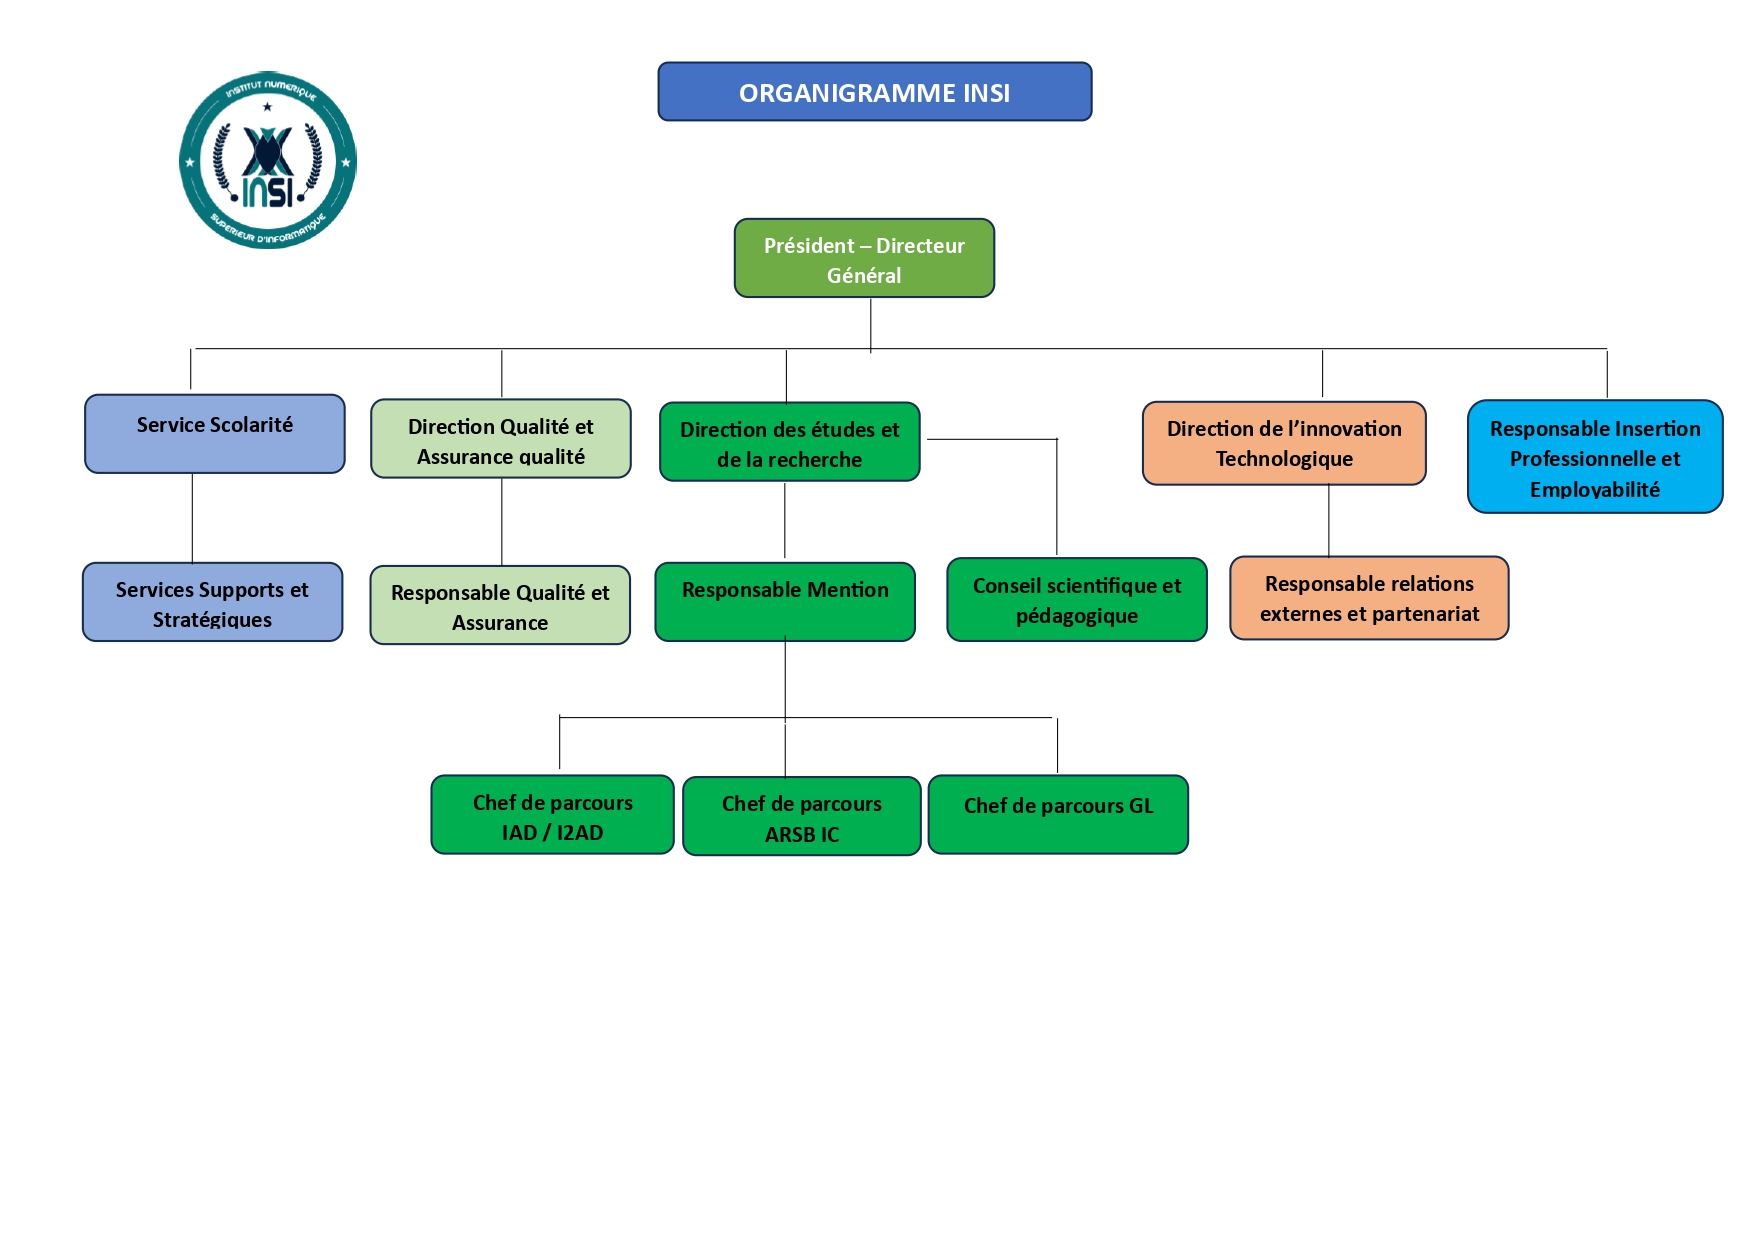
\includegraphics[width=12cm]{organigramme.jpg}
    \caption{Organigramme de l’INSI }
    \textit{Source : INSI, 2025}
    \label{fig:organigramme}
\end{figure}


L'organigramme de l’INSI, en partenariat avec le Collège de Paris, est structuré autour d’une direction générale incarnée par le Président Directeur Général. Ce dernier assure la coordination de trois pôles principaux : la \textbf{Direction Administrative et Financière}, la \textbf{Direction des Études}, et le \textbf{Service des Relations Internationales et Mobilités}.

Le \textbf{Président Directeur Général} assure la direction stratégique de l’institut. Il supervise l’ensemble des activités pédagogiques, administratives et de développement. Il veille à la qualité de l’enseignement, à la bonne gestion des ressources humaines et matérielles, et représente l’établissement auprès des partenaires et autorités.

La \textbf{Direction Administrative et Financière} est chargée de la gestion des affaires internes, notamment à travers deux services essentiels : 
\begin{itemize}
    \item le \textbf{Service des scolarités}, qui s’occupe des dossiers étudiants, inscriptions et suivi académique,
    \item les \textbf{Services supports et stratégiques}, qui assurent un appui logistique, administratif et technologique à l’ensemble de l’institut.
\end{itemize}

Le \textbf{pôle des Relations Internationales et Mobilités} gère les échanges académiques avec l’étranger ainsi que les projets de mobilité étudiante ou enseignante. 

La \textbf{Direction des Études} supervise quant à elle l’ensemble des programmes pédagogiques et le corps enseignant. Elle travaille en étroite collaboration avec un \textbf{Responsable Parcours}, qui coordonne les différentes spécialisations proposées. Cette direction intègre également une \textbf{cellule Formation professionnelle et certification}, en charge des dispositifs de validation des compétences, des certifications professionnelles et des parcours de formation continue. Elle comprend aussi le \textbf{Département alternance et emplois}, responsable du suivi des étudiants en contrat d’alternance, des stages professionnels, et de l’insertion professionnelle.

Sous la responsabilité du \textbf{Responsable Parcours}, plusieurs responsables pédagogiques gèrent les différentes filières de formation :
\begin{itemize}
    \item le \textbf{parcours tronc commun}, qui regroupe les matières fondamentales partagées par tous les étudiants en début de cycle,
    \item le \textbf{parcours ARSB \& IC},
    \item le \textbf{parcours GL \& MSI},
    \item le \textbf{parcours IAD \& I2AD}.
\end{itemize}

D’autres structures, bien que non représentées sur cet organigramme, contribuent également de manière significative à la mission de l’INSI :
\begin{itemize}
    \item Le \textbf{Conseil de l’École}, regroupant des membres de l’équipe pédagogique et administrative. Il joue un rôle consultatif ou décisionnel sur les questions académiques : validation des programmes, suivi des résultats, discipline, méthodologie, etc.
    \item Le \textbf{Responsable de la formation en ligne}, qui conçoit et supervise les dispositifs d’apprentissage à distance. Il s’assure que les contenus en ligne sont accessibles, interactifs et conformes aux standards pédagogiques, tout en accompagnant enseignants et étudiants dans leur utilisation.
    \item L’\textbf{Association et les clubs étudiants}, qui encadrent et soutiennent les initiatives étudiantes, les clubs thématiques (informatique, innovation, sport, culture, etc.), et les événements organisés dans le cadre de la vie étudiante. Cela favorise l’engagement, le développement personnel et les compétences transversales des étudiants.
\end{itemize}

Cette structure témoigne d’une organisation à la fois pédagogique, administrative et tournée vers l’international et l’employabilité, assurant une formation complète et professionnalisante aux étudiants.
\subsection{Domaine de spécialisation}

INSI University propose des parcours académiques professionnalisants dans le domaine de l’informatique et des technologies numériques, articulés autour de licences professionnelles, de masters spécialisés, de formations professionnelles continues et d’opportunités de mobilité internationale.

\subsubsection{Licences professionnelles}

Les programmes de licence offrent une formation de base solide, axée sur la pratique, et préparant à une insertion rapide dans le monde professionnel :

\begin{itemize}
    \item \textbf{GL (Génie Logiciel)} : Conception, développement et maintenance d'applications logicielles.
    \item \textbf{ARSB (Administration Réseaux et Systèmes et Base de données)} : Gestion d’infrastructures informatiques, réseaux, serveurs et systèmes.
    \item \textbf{IAD (Intelligence Artificielle et Data Science)} : Introduction aux algorithmes d’IA, au traitement de données et à l’apprentissage automatique.
\end{itemize}

\subsubsection{Masters professionnels}

Les masters permettent d’approfondir les compétences techniques et managériales, en lien étroit avec les évolutions du secteur :

\begin{itemize}
    \item \textbf{MSI (Management des Systèmes d’Information)} : Pilotage de projets numériques, gouvernance des SI.
    \item \textbf{IC (Infrastructures et Cybersécurités)} : Sécurisation des systèmes, audit, réseaux avancés.
    \item \textbf{I2AD (Intelligence Artificielle, Analyse de Données et Automatisation)} : Applications avancées de l’IA, automatisation des processus et science des données.
\end{itemize}

\subsubsection{Formations professionnelles continues}

INSI University propose également des formations professionnelles continues, spécifiquement conçues pour les professionnels déjà en poste souhaitant approfondir leurs compétences ou se spécialiser dans l’un des domaines proposés.

Ces formations sont adaptées aux contraintes des professionnels (horaires flexibles, modules pratiques) et visent à renforcer leur employabilité ou à accompagner leur évolution de carrière.

\subsubsection{Mobilité internationale et double diplôme}

Dans une optique d’ouverture et de reconnaissance internationale, INSI propose à ses étudiants des opportunités de mobilité académique et de double diplôme, à partir de la deuxième année (L2) :

\begin{itemize}
    \item \textbf{Format hybride} : 6 mois de formation à Madagascar + 6 mois à l’étranger selon le parcours choisi.
    \item \textbf{Double diplôme en L3 ou M2} : En partenariat avec des institutions internationales telles que :
    \begin{itemize}
        \item Collège de Paris (France)
        \item Keyce Informatique (France)
        \item Eskills (Québec, Canada)
    \end{itemize}
\end{itemize}

\subsubsection*{Conditions d’éligibilité}
\begin{itemize}
    \item Niveau DALF C1 en français pour la mobilité vers des pays francophones.
    \item Niveau B2 ou C1 en anglais pour les destinations anglophones.
\end{itemize}

\subsection{Architectures des formations pédagogiques}

Le recrutement des étudiants à l’INSI s’effectue exclusivement par sélection de dossiers pour l’entrée en première année de Licence (L1), et par voie de concours pour l’admission en Master 1.

Au sein de l’INSI, une seule mention est proposée : \textbf{Informatique}, déclinée en trois parcours distincts aux niveaux Licence et Master.


\begin{table}[H]
\centering
\begin{tabular}{|l|l|}
\hline
\textbf{Licence} & \textbf{Master} \\
\hline
Génie Logiciel (GL) & Management des Systèmes d’Information (MSI) \\
\hline
Administration Réseaux, Systèmes et Bases de \\données (ARSB) & Infrastructures et Cybersécurités (IC) \\
\hline
Intelligence Artificielle et Data Science (IAD) & Intelligence Artificielle, Analyse de Données et \\Automatisation (I2AD) \\
\hline
\end{tabular}
\caption{Parcours Licence et Master proposés à l’INSI}
\textit{Source : INSI, 2025}
\label{tab:parcours}
\end{table} 

L’architecture des études à trois niveaux conformément au système LMD (Licence Master et Doctorat) permet les comparaisons et les équivalences académiques des diplômes au niveau international.\\
L = Licence (Bac + 3) = L1, L2, L3 = 6 semestres S1 à S6\\
M = Master (Bac + 5) = M1, M2 = 4 semestres S7 à S10\\
Le diplôme de licence est obtenu en 3 années des études après Baccalauréat. Et le diplôme de Master est obtenu en 2 ans après obtenu du diplôme de LICENCE.\\
Le MASTER PROFESSIONNEL est un diplôme destiné à la recherche emploi au terme des études.\\

\textbf{Spécificités pédagogiques} 
\begin{itemize}
    \item École d'alternance dès la L2 S4\\
    Alternance cours/entreprise pour une meilleure insertion
    \item Écoles connectées \& e-learning\\
    Plateforme numérique de formation, cloud intégré, Google Workspace\\
    Cours accessibles en ligne selon les parcours
    \item Pédagogie active \& par projets\\
    Hackathons, soutenances exposées, projets réels en entreprise
\end{itemize}

\subsubsection{Relations de l’INSI avec les entreprises et les organismes} 
L’Institut National Supérieur en Informatique (INSI) entretient des liens étroits avec le monde professionnel. L’INSI collabore activement avec de nombreux organismes publics, semi-publics et privés, tant au niveau national qu’international. Cette collaboration se traduit concrètement par l’organisation régulière de stages obligatoires pour les étudiants, favorisant leur immersion professionnelle et leur employabilité.\\

Parmi les entreprises et institutions partenaires accueillant nos étudiants en stage chaque année :
\begin{itemize}
    \item Data Pulse Center
    \item RELIA Consulting
    \item Code Talent
    \item Bocasay
    \item Minimad
    \item Smartone AI
    \item NOVITY
    \item Eclosia Madagascar
    \item VISEO Groupe
    \item Océane Trade
    \item ACCES Banque
\end{itemize}

En plus des stages, l’INSI organise régulièrement des visites pédagogiques, des rencontres métiers et des projets collaboratifs avec plusieurs entreprises du secteur technologique et numérique. Ces activités permettent aux étudiants de mieux comprendre les réalités du terrain, d’échanger avec des professionnels et de s’ouvrir à l’environnement entrepreneurial.\\

Parmi les entreprises ayant accueilli ces initiatives :
\begin{itemize}
    \item NOVITY
    \item YAS Madagascar
    \item Smartone AI
    \item Eclosia Madagascar
    \item et d'autres acteurs majeurs du numérique à Madagascar
\end{itemize}

Cette dynamique de partenariat permanent constitue un pilier de la pédagogie à l’INSI, en lien avec son objectif de former des professionnels compétents, opérationnels et ancrés dans les besoins du marché.\\

\subsubsection{Partenariat au niveau international} 
L’INSI s’est inscrit dans une dynamique d’ouverture à l’international grâce à son partenaire fondateur, ILO Madagascar, représentant de l’Organisation Internationale du Travail. Cette orientation se renforce aujourd’hui à travers des partenariats stratégiques avec des institutions académiques et des entreprises internationales, permettant à l’Institut de proposer une formation alignée sur les standards mondiaux.\\

L’INSI bénéficie actuellement de programmes de co-diplomation et de double diplôme en collaboration avec plusieurs établissements internationaux de renom :
\begin{itemize}
    \item Collège de Paris International
    \item Keyce Informatique (France)
    \item Eskills Academy (Québec, Canada)
    \item École Supérieure Polytechnique d’Antsiranana (ESPA) – pour une synergie régionale renforcée
\end{itemize}

Par ailleurs, à travers les stages annuels et projets pédagogiques, l’INSI collabore également avec des entreprises à dimension régionale ou mondiale :
\begin{itemize}
    \item VISEO Groupe
    \item Eclosia Madagascar (Groupe mauricien)
    \item Smartone AI
    \item NOVITY
\end{itemize}

\subsubsection{Parcours professionnels des diplômés} 
Les diplômés de la Licence en Informatique de l’INSI disposent d’un socle solide de compétences en programmation, systèmes, réseaux, bases de données et développement logiciel. Cette polyvalence leur permet d’intégrer directement le marché du travail ou de poursuivre en Master. À ce niveau, ils peuvent exercer en tant que :
\begin{itemize}
    \item Technicien système et réseau
    \item Développeur web / mobile (front-end ou back-end)
    \item Administrateur systèmes junior
    \item Technicien support IT
    \item Intégrateur / testeur logiciel
    \item Assistant en sécurité informatique
    \item Assistant en projets d’IA ou de data (selon profil)
\end{itemize}

Les stages annuels en entreprise leur offrent une première expérience professionnelle valorisante dans des structures variées : entreprises technologiques, banques, administrations, startups, ONG, etc.\\

La formation de Master proposée à l’INSI, grâce à ses parcours spécialisés, forme des professionnels capables d’intervenir sur des projets complexes, innovants et à dimension stratégique. Les débouchés varient selon la spécialisation choisie :

\textbf{Parcours Ingénierie logicielle, réseaux et systèmes :}
\begin{itemize}
    \item Ingénieur en développement logiciel / full-stack
    \item Architecte logiciel
    \item Ingénieur systèmes et réseaux
    \item Administrateur cloud / DevOps
    \item Chef de projet informatique
\end{itemize}

\textbf{Parcours Cybersécurité :}
\begin{itemize}
    \item Expert en sécurité des systèmes d'information
    \item Analyste SOC / CERT
    \item Auditeur en cybersécurité
    \item Responsable de la sécurité IT (RSSI)
\end{itemize}

\textbf{Parcours Intelligence Artificielle et Data :}
\begin{itemize}
    \item Data Scientist
    \item Data Analyst
    \item Ingénieur en Intelligence Artificielle
    \item Machine Learning Engineer
    \item Développeur d'applications intelligentes
    \item Consultant en IA
    \item Spécialiste en traitement automatique du langage naturel (TALN)
    \item Spécialiste en vision par ordinateur (Computer Vision)
\end{itemize}

Grâce aux partenariats internationaux et aux projets en entreprise, les diplômés du Master peuvent également prétendre à des postes dans des structures multinationales, ou poursuivre une carrière académique et de recherche (doctorat, enseignement supérieur).\\

\subsubsection{Ressources humaines} 
L’INSI s’appuie sur une équipe pédagogique et administrative compétente, dynamique et engagée dans la réussite de ses étudiants. Ses ressources humaines se répartissent comme suit :
\begin{itemize}
    \item Président Directeur de l’INSI : Dr RAMASONDRANO Andriamanjaka
    \item Responsable parcours ARSB \& IC : Mr RATIANARISON Hery Mampionona
    \item Responsable parcours tronc commun : Dr RAKOTONDRAMANANA R, Sitraka
    \item Responsable parcours GL \& MSI : Mr ANDRIAMIADANA TANTELY ANTOINE
    \item Responsable parcours IAD \& I2AD : par intérim PDG
    \item Nombres d'enseignants : 40
    \item Nombres des personnels administratives : 04
    \item Personnels d’appui : 6
\end{itemize}

\vfill*{}
\newpage

\section{État de l'art et Cadre théorique}
\subsection{Contexte et analyse sectorielle de la rizipisciculture à Madagascar}
Le tilapia est l'une des espèces les plus élevées dans le monde, car il s'adapte facilement à différents environnements. La rizipisciculture est une pratique qui consiste à associer l'élevage de poissons à la culture du riz dans les mêmes parcelles. Cette technique est utilisée depuis le milieu du XX\textsuperscript{ème} siècle et présente un avantage simple : le riz protège les poissons et leur sert de nourriture, tandis que les poissons fertilisent naturellement les rizières. Des études réalisées sur les Hautes-Terres malgaches par l'APDRA montrent que l'ajout de poissons dans une rizière peut augmenter le rendement du riz de 10 \% à 20 \%, sans réduire la surface cultivable.\\

Pour situer ce sujet, plusieurs aspects peuvent être analysés. Du côté politique, l'État malgache met en place une stratégie de modernisation numérique de l'agriculture. La Stratégie Nationale de Transformation Digitale de l'Agriculture (2024-2028), portée par le Ministère de l'Agriculture et de la Souveraineté Alimentaire avec le Ministère du Développement Numérique, prévoit la mise en place d'une Infrastructure Publique Numérique Agricole. Cette infrastructure doit relier les différents acteurs du secteur (institutions publiques, instituts de recherche comme le FOFIFA, organisations de producteurs) et garantir que les données agricoles restent maîtrisées par le pays. Cette stratégie est aussi soutenue par des partenaires comme la Banque mondiale et la FAO.\\

Du côté économique, la rizipisciculture permet aux paysans d'obtenir deux produits (riz et poisson) sur la même parcelle, pour un coût d'installation réduit, ce qui en fait une source de revenu supplémentaire intéressante.\\

Du côté socioculturel, la rizipisciculture est une pratique ancienne à Madagascar utilisée par les paysans à travers le pays. Le tilapia est bien connu et apprécié par les consommateurs locaux, notamment parce qu'il grandit vite. Pourtant, la grande majorité des riziculteurs malgaches cultivent uniquement le riz et ne pratiquent pas l'élevage de tilapia dans leurs parcelles, souvent par manque de connaissance de la pratique ou par manque d'outils pour la mener sereinement.\\

Du côté technologique, l'usage de capteurs et de modèles de machine learning pour surveiller la qualité de l'eau se développe déjà dans l'aquaculture intensive à l'échelle mondiale. Mais à Madagascar, ces outils sont encore peu utilisés dans la rizipisciculture, où le suivi de l'eau se fait encore principalement à l'œil ou de façon manuelle.\\

Du côté environnemental, la rizipisciculture est considérée comme un système de production qui a un faible impact écologique. IISD affirme une réduction des émissions de gaz à effet de serre d'environ 0,81 kg de CO\textsubscript{2} équivalent par kilogramme de riz produit, par rapport à des systèmes de pisciculture plus intensifs. Mais la qualité de l'eau dans une parcelle rizipiscicole peut varier rapidement (température, oxygène, nutriments), et si ces variations ne sont pas surveillées et anticipées, elles peuvent mettre en danger les poissons élevés.\\

Enfin, du côté légal, le développement de l'aquaculture à Madagascar est encadré depuis le milieu des années 2000 par une stratégie nationale de développement durable de l'aquaculture, mise en place par le Ministère chargé de la Pêche avec la FAO. Plus récemment, la feuille de route de l'Infrastructure Publique Numérique Agricole insiste sur la gouvernance et la maîtrise des données du secteur.\\

Face à ces défis environnementaux et techniques, l'application de l'intelligence artificielle offre une opportunité de suivi automatisé.

\subsection{Fondements théoriques des modèles d'apprentissage et de traitement de données}

Après avoir situé le contexte sectoriel de la rizipisciculture, il est nécessaire de poser les bases théoriques des outils qui seront utilisés dans ce mémoire. Cette section présente d'abord les algorithmes de machine learning mobilisés pour les tâches de régression et de classification, ainsi que la méthode d'optimisation retenue, puis les techniques d'analyse temporelle et de deep learning utilisées pour la prédiction à court terme de la qualité de l'eau.\\

\subsubsection{Algorithmes de Machine Learning}
\paragraph{Régression Linéaire\\}

La régression linéaire est le modèle le plus simple pour prédire une valeur numérique continue à partir d'un ensemble de variables explicatives. Le modèle suppose qu'il existe une relation linéaire entre les variables d'entrée ( $x_1, x_2, \dots, x_n$ ) et la variable de sortie ( y ). Pour une observation donnée, la prédiction ( $\hat{y}$ ) s'écrit :
\[
\hat{y} = \beta_0 + \beta_1 x_1 + \beta_2 x_2 + \dots + \beta_n x_n
\]
où :\\
$\hat{y}$ est la valeur prédite\\
$\beta_0$ est l'ordonnée à l'origine (biais), c'est-à-dire la valeur prédite lorsque toutes les variables d'entrée sont nulles\\
$\beta_1, \dots, \beta_n$ sont les coefficients associés à chaque variable, indiquant le poids et le sens de l'influence de chaque caractéristique du sol sur la densité prédite.\\

\begin{table}[H]
\centering
\begin{tabular}{|m{5cm}|m{12cm}|}
\hline
\textbf{Hyperparamètre} & \textbf{Interprétation} \\
\hline
\texttt{fit\_intercept} & Indique si le modèle doit calculer l'ordonnée à l'origine $\beta_0$, ou la fixer à zéro. \texttt{True} : le biais est estimé normalement. \newline \texttt{False} : le modèle est contraint à passer par l'origine, ce qui n'est pertinent que si l'on sait a priori que $y=0$ lorsque toutes les variables sont nulles. \\
\hline
\end{tabular}
\caption{Hyperparamètres -- Régression Linéaire}
\textit{Source : Réalisation Personnelle}
\end{table}

\paragraph{Régression Logistique\\}
Contrairement à la régression linéaire, la régression logistique n'est pas utilisée pour prédire une valeur continue, mais pour résoudre un problème de classification.\\
La régression logistique résout ce problème en appliquant une fonction supplémentaire à la combinaison linéaire des variables : la fonction sigmoïde, notée $ \sigma $, qui transforme n'importe quelle valeur réelle en une valeur comprise entre 0 et 1, interprétable comme une probabilité :
\[
\sigma(z) = \frac{1}{1 + e^{-z}}
\]
En posant $ z = \beta_0 + \beta_1 x_1 + \dots + \beta_n x_n $, la probabilité que l'observation appartienne à la classe positive s'écrit :
\[
P(y = 1 \mid x) = \sigma(z) = \frac{1}{1 + e^{-(\beta_0 + \beta_1 x_1 + \dots + \beta_n x_n)}}
\]

\begin{longtable}{|m{5cm}|m{12cm}|}
\hline
\textbf{Hyperparamètre} & \textbf{Interprétation} \\
\hline
\texttt{C} & Inverse de la force de régularisation : une valeur faible impose une forte régularisation, une valeur élevée laisse le modèle s'ajuster plus librement aux données. \\
\hline
\texttt{penalty} & Type de régularisation appliquée aux coefficients.\newline\texttt{l2} : pénalise le carré des coefficients, les réduit sans les annuler \newline\texttt{l1} : pénalise leur valeur absolue, ce qui peut annuler certains coefficients (sélection de variables) \newline \texttt{elasticnet} : combinaison pondérée de l1 et l2 \newline \texttt{none} : aucune régularisation appliquée. \\
\hline
\texttt{solver} & Algorithme d'optimisation utilisé pour minimiser la fonction de coût logistique.\newline \texttt{lbfgs} : méthode quasi-Newton, adaptée aux jeux de données de taille moyenne avec pénalité l2 \newline \texttt{liblinear} : adapté aux petits jeux de données et compatible avec la pénalité l1 \newline \texttt{saga} : adapté aux grands jeux de données et compatible avec l1, l2 et elasticnet \newline \texttt{newton-cg} et \texttt{sag} : variantes alternatives d'optimisation, plus rapides sur de grands volumes de données avec pénalité l2. \\
\hline
\texttt{max\_iter} & Nombre maximal d'itérations autorisées à l'algorithme d'optimisation pour converger vers une solution. \\
\hline
\caption{Hyperparamètres -- Régression Logistique}
\end{longtable}
\begin{center}
\vspace{-0.85cm}
\textit{Source : Réalisation Personnelle}
\end{center}


\paragraph{Machines à Vecteurs de Support (SVM)\\}
Les Machines à Vecteurs de Support cherchent à séparer les données en deux classes en traçant un hyperplan (une droite, ou son équivalent en plusieurs dimensions) entre elles. Parmi tous les hyperplans possibles, le SVM choisit celui qui maximise la marge, c'est-à-dire la distance entre l'hyperplan et les points les plus proches de chaque classe, appelés vecteurs de support :
\[
f(x) = \mathbf{w}^T x + b
\]
où $\mathbf{w}$ et $b$ définissent la position et l'orientation de l'hyperplan. Un hyperplan qui maximise cette marge généralise en principe mieux sur de nouvelles données. Lorsque les données ne sont pas séparables par une simple droite, le SVM utilise l'astuce du noyau (kernel trick), qui permet de les séparer comme si elles avaient été projetées dans un espace de dimension supérieure, sans avoir à calculer cette projection. Le SVM se décline en deux variantes : le SVC pour la classification et le SVR pour la régression.

\begin{longtable}{|m{5cm}|m{12cm}|}
\hline
\textbf{Hyperparamètre} & \textbf{Interprétation} \\
\hline
\texttt{C} & Contrôle le compromis entre la maximisation de la marge et la tolérance aux erreurs de classification. \\
\hline
\texttt{kernel} & Type de noyau utilisé pour séparer les données. \newline \texttt{linear} : suppose une séparation linéaire des données, sans transformation \newline \texttt{poly} : introduit des combinaisons polynomiales des variables, utile pour des frontières courbes simples \newline \texttt{rbf} (par défaut) : noyau gaussien, adapté à des frontières de décision complexes et non linéaires. \\
\hline
\texttt{gamma} & Dans le noyau RBF, contrôle l'influence de chaque point d'entraînement sur la frontière de décision. \\
\hline
\texttt{epsilon} (SVR) & Définit la largeur du tube de tolérance autour des prédictions, à l'intérieur duquel aucune pénalité n'est appliquée. \\
\hline
\caption{Hyperparamètres -- SVM}
\end{longtable}
\begin{center}
\vspace{-0.85cm}
\textit{Source : Réalisation Personnelle}
\end{center}

\paragraph{Arbre de Décision\\}
L'Arbre de Décision construit une succession de règles de décision simples sous forme d'arbre. À chaque nœud, une question binaire est posée sur une variable , ce qui dirige l'observation vers l'enfant de gauche ou de droite, jusqu'à atteindre une feuille contenant la prédiction finale. Le découpage à chaque nœud est choisi selon un critère d'homogénéité, mesuré principalement de deux façons en classification :

L'impureté de Gini, qui mesure la probabilité de mal classer une observation si elle était étiquetée aléatoirement selon la distribution des classes du nœud :
\[
G = 1 - \sum_{k=1}^{K} p_k^2
\]

L'Entropie, issue de la théorie de l'information, qui mesure le désordre ou l'incertitude présente dans le nœud :
\[
H = - \sum_{k=1}^{K} p_k \log_2(p_k)
\]

où $p_k$ est la proportion d'observations de la classe $k$ dans le nœud considéré. Dans les deux cas, une valeur de 0 correspond à un nœud parfaitement homogène (une seule classe présente), tandis que la valeur est maximale lorsque les classes sont réparties de façon égale dans le nœud.

\begin{longtable}{|m{5cm}|m{12cm}|}
\hline
\textbf{Hyperparamètre} & \textbf{Interprétation} \\
\hline
\texttt{max\_depth} & Profondeur maximale de l'arbre : une valeur élevée capture des relations plus complexes mais augmente le risque de surapprentissage. \\
\hline
\texttt{min\_samples\_split} & Nombre minimal d'observations requises dans un nœud pour autoriser un nouveau découpage. \\
\hline
\texttt{min\_samples\_leaf} & Nombre minimal d'observations requises dans une feuille. \\
\hline
\texttt{criterion} & Critère utilisé pour évaluer la qualité d'un découpage. \newline En classification : \newline \texttt{gini} mesure la probabilité de mal classer une observation tirée au hasard selon la distribution du nœud \newline \texttt{entropy} mesure le désordre des classes présentes, avec une pénalisation légèrement plus forte des nœuds très mélangés.\newline En régression : \newline \texttt{squared\_error} (erreur quadratique) est le critère standard \newline \texttt{absolute\_error} est moins sensible aux valeurs extrêmes \newline \texttt{friedman\_mse} est une variante de l'erreur quadratique optimisée pour les découpages successifs. \\
\hline
\texttt{ccp\_alpha} & Paramètre de complexité utilisé pour l'élagage (pruning) de l'arbre après sa construction : plus sa valeur est élevée, plus les branches apportant peu de gain sont supprimées, ce qui limite le surapprentissage. \\
\hline
\texttt{max\_features} & Nombre de variables considérées lors de la recherche du meilleur découpage à chaque nœud :\newline \texttt{None} (toutes les variables), \newline \texttt{sqrt} ou \texttt{log2} (un sous-ensemble restreint), ce qui introduit de la variabilité entre les découpages. \\
\hline
\caption{Hyperparamètres -- Arbre de Décision}
\end{longtable}
\begin{center}
\vspace{-0.85cm}
\textit{Source : Réalisation Personnelle}
\end{center}

\paragraph{Random Forest\\}
La Random Forest combine un grand nombre d'arbres de décision entraînés sur des échantillons différents des données , et sur un sous-ensemble aléatoire des variables à chaque nœud. Cette double source d'aléa décorrèle les arbres entre eux et réduit la variance globale du modèle. Les prédictions sont ensuite combinées différemment selon la tâche :
\[
\hat{y} = \text{mode}\left(\hat{y}^{(1)}, \dots, \hat{y}^{(T)}\right) \quad \text{(classification, vote majoritaire)}
\]
\[
\hat{y} = \frac{1}{T}\sum_{t=1}^{T} \hat{y}^{(t)} \quad \text{(régression, moyenne des arbres)}
\]



\begin{longtable}{|m{5cm}|m{12cm}|}
\hline
\textbf{Hyperparamètre} & \textbf{Interprétation} \\
\hline
\texttt{n\_estimators} & Nombre d'arbres constituant la forêt : plus il y en a, plus la variance du modèle est réduite, au prix d'un temps de calcul plus long. \\
\hline
\texttt{max\_depth} & Profondeur maximale de chaque arbre de la forêt. \\
\hline
\texttt{max\_features} & Nombre de variables tirées aléatoirement à considérer à chaque nœud. \newline \texttt{sqrt} : considère la racine carrée du nombre total de variables (valeur courante en classification) \newline \texttt{log2} : considère le logarithme en base 2 du nombre total de variables, un choix plus restrictif \newline\texttt{None} : considère l'ensemble des variables à chaque nœud, ce qui réduit la décorrélation entre les arbres. \\
\hline
\texttt{min\_samples\_split} & Nombre minimal d'observations requises dans un nœud pour autoriser un nouveau découpage, appliqué à chaque arbre de la forêt. \\
\hline
\caption{Hyperparamètres -- Random Forest\\}
\end{longtable}
\begin{center}
\vspace{-0.7cm}
\textit{Source : Réalisation Personnelle}
\end{center}

\paragraph{XGBoost (Extreme Gradient Boosting)\\}
XGBoost est également un algorithme basé sur des arbres de décision, mais il repose sur un principe différent. Plutôt que d'entraîner les arbres indépendamment les uns des autres, XGBoost les construit de manière séquentielle, chaque nouvel arbre étant entraîné pour corriger les erreurs commises par l'ensemble des arbres précédents. La prédiction finale est la somme pondérée des prédictions de tous les arbres construits :
\[
\hat{y} = \sum_{t=1}^{T} f_t(x)
\]
où chaque $f_t$ est un arbre de décision entraîné à corriger l'erreur résiduelle laissée par les arbres $f_1, \dots, f_{t-1}$. Ce fonctionnement séquentiel et cette correction intégrée expliquent pourquoi XGBoost obtient souvent de meilleures performances, aussi bien pour des tâches de régression (la sortie $\hat{y}$ est directement une valeur continue) que pour des tâches de classification (la somme des arbres est passée dans une fonction sigmoïde, comme pour la régression logistique, afin d'obtenir une probabilité de classe), au prix d'un temps d'entraînement plus long et d'un réglage plus sensible de ses hyperparamètres.

\begin{longtable}{|m{5cm}|m{12cm}|}
\hline
\textbf{Hyperparamètre} & \textbf{Interprétation} \\
\hline
\texttt{n\_estimators} & Nombre d'arbres construits séquentiellement lors du Boosting. \\
\hline
\texttt{learning\_rate} & Poids appliqué à la contribution de chaque nouvel arbre : une valeur faible ralentit l'apprentissage mais le rend plus stable. \\
\hline
\texttt{max\_depth} & Profondeur maximale de chaque arbre, contrôlant la complexité des corrections apportées à chaque étape. \\
\hline
\texttt{min\_child\_weight} & Somme minimale des poids des observations requise dans un nœud enfant pour qu'un découpage soit effectué ; une valeur plus élevée rend le modèle plus conservateur et limite le surapprentissage sur des groupes d'observations trop petits. \\
\hline
\texttt{gamma} & Réduction minimale de la fonction de perte requise pour justifier un nouveau découpage d'une feuille ; plus sa valeur est élevée, plus l'algorithme est prudent avant de complexifier l'arbre. \\
\hline
\caption{Hyperparamètres -- XGBoost\\}
\end{longtable}
\begin{center}
\vspace{-0.85cm}
\textit{Source : Réalisation Personnelle}
\end{center}

\subsubsection{Analyse Temporelle et Deep Learning}
\paragraph{Décomposition STL\\}
La décomposition STL (Seasonal-Trend decomposition using Loess) est une méthode qui permet de décomposer une série temporelle en trois composantes distinctes : la tendance, la saisonnalité et le résidu. Une série temporelle $Y_t$ s'écrit ainsi :
\[
Y_t = T_t + S_t + R_t
\]
où $T_t$ est la tendance (évolution générale de la série sur le long terme), $S_t$ la composante saisonnière (variations qui se répètent à intervalles réguliers) et $R_t$ le résidu, c'est-à-dire les fluctuations restantes non expliquées par les deux premières composantes. Comme son nom l'indique, cette décomposition repose sur la méthode de lissage Loess, appliquée successivement pour extraire chacune de ces trois composantes à partir de la série brute.
\subparagraph{La méthode Loess\\}
Loess (Locally Estimated Scatterplot Smoothing) est une méthode de lissage qui estime une courbe régulière à partir de données bruitées, sans supposer de forme mathématique globale. Pour estimer la valeur lissée en un point $x_0$, seules les observations voisines sont utilisées, chacune pondérée selon sa proximité, généralement via une fonction tricube :
\[
w_i = \left(1 - \left|\frac{x_i - x_0}{d}\right|^3\right)^3
\]
où $d$ est la distance au point voisin le plus éloigné inclus dans le voisinage considéré. Plus une observation $x_i$ est proche de $x_0$, plus son poids $w_i$ est élevé. Une régression pondérée est ensuite ajustée sur ce voisinage, en minimisant l'erreur quadratique pondérée :
\[
\min_{\beta} \sum_{i} w_i \left(y_i - \beta_0 - \beta_1 x_i\right)^2
\]
et seule sa valeur en $x_0$ est retenue comme estimation lissée. Ce calcul est répété en glissant le voisinage le long de la série, ce qui produit une courbe qui s'adapte localement aux données.

Dans la décomposition STL, Loess est appliqué successivement : d'abord pour estimer la tendance $T_t$ (variations lentes), puis pour extraire la saisonnalité $S_t$ à partir des données privées de cette tendance, le résidu $R_t$ étant ce qui reste après soustraction des deux composantes.

\paragraph{Réseaux LSTM\\}
Les modèles de machine learning classiques (régression, SVM, arbres de décision) traitent chaque observation de manière indépendante et ne conservent aucune mémoire des observations précédentes. Cette limite les rend peu adaptés aux données séquentielles, comme une série temporelle, où la valeur à un instant donné dépend fortement des valeurs passées.

Les réseaux de neurones récurrents (RNN) ont été conçus pour ce type de données : à chaque instant $t$, ils combinent l'entrée courante avec une information héritée de l'étape précédente, ce qui leur permet de propager un contexte d'une étape à l'autre. Cependant, sur une séquence longue, cette information a tendance à s'atténuer au fil des étapes, jusqu'à disparaître presque complètement. C'est le problème de la disparition du gradient (vanishing gradient), qui empêche le RNN classique de retenir une information sur de longues séquences.

Les réseaux LSTM (Long Short-Term Memory) ont été conçus pour résoudre ce problème. L'idée centrale est d'ajouter une mémoire à long terme, appelée état de la cellule $C_t$, qui circule d'une étape à l'autre en étant peu modifiée, ce qui lui permet de conserver une information sur de longues séquences sans qu'elle ne s'efface. L'accès à cette mémoire est contrôlé par trois portes (gates), chacune étant une couche de neurones à activation sigmoïde $\sigma$, qui produit une valeur entre 0 (« bloquer ») et 1 (« laisser passer »), et qui décident respectivement :

\begin{itemize}
\item la \textbf{porte d'oubli}, quelle partie de la mémoire passée doit être conservée ou supprimée :
\[
f_t = \sigma(W_f \cdot [h_{t-1}, x_t] + b_f)
\]
\item la \textbf{porte d'entrée}, quelle nouvelle information, apportée par l'observation courante, doit être ajoutée à cette mémoire :
\[
i_t = \sigma(W_i \cdot [h_{t-1}, x_t] + b_i)
\]
\item la \textbf{porte de sortie}, quelle partie de cette mémoire doit être transmise comme résultat à l'instant courant, et servir de base pour l'étape suivante :
\[
o_t = \sigma(W_o \cdot [h_{t-1}, x_t] + b_o)
\]
\end{itemize}

où $x_t$ est l'entrée à l'instant $t$, $h_{t-1}$ l'état caché de l'étape précédente, et $W$, $b$ les poids et biais propres à chaque porte. La mémoire de la cellule est ensuite mise à jour en combinant ce qui a été conservé de l'ancienne mémoire et ce que la porte d'entrée autorise à ajouter :
\[
C_t = f_t \odot C_{t-1} + i_t \odot \tanh(W_C \cdot [h_{t-1}, x_t] + b_C)
\]
où $\odot$ désigne une multiplication élément par élément. Enfin, l'état caché transmis à l'étape suivante est obtenu en filtrant cette mémoire mise à jour à travers la porte de sortie :
\[
h_t = o_t \odot \tanh(C_t)
\]

Chaque porte est une petite couche de neurones qui produit une valeur entre 0 et 1, agissant comme un filtre : une valeur proche de 0 bloque l'information, une valeur proche de 1 la laisse passer. Grâce à ce mécanisme, la cellule LSTM peut choisir de garder une information pertinente sur de nombreuses étapes, ou de l'oublier rapidement si elle ne l'est plus, ce qui permet au réseau de capter des dépendances temporelles aussi bien courtes que longues, sans souffrir de la disparition du gradient qui limite les RNN classiques.

\subsubsection{Optimisation par GridSearch}

Il faut distinguer les paramètres d'un modèle, qui sont appris automatiquement pendant l'entraînement, des hyperparamètres, qui sont fixés avant l'entraînement et qui contrôlent le comportement général du modèle.

Le choix de ces hyperparamètres influence fortement la performance d'un modèle, mais il n'existe pas de formule directe pour les déterminer : ils doivent être testés empiriquement. Le GridSearch (recherche par grille) consiste à définir, pour chaque hyperparamètre, un ensemble de valeurs candidates, puis à tester méthodiquement toutes les combinaisons possibles entre ces valeurs.

Pour évaluer chaque combinaison de façon fiable, le GridSearch est combiné à une validation croisée (cross-validation). Cette technique divise les données d'entraînement en $k$ sous-ensembles (folds) de taille égale ; le modèle est entraîné $k$ fois, en utilisant à chaque fois $k-1$ folds pour l'entraînement et le fold restant pour l'évaluation, puis les $k$ scores obtenus sont moyennés :
\[
\text{Score}_{CV} = \frac{1}{k}\sum_{i=1}^{k} \text{Score}_i
\]

La combinaison d'hyperparamètres obtenant le meilleur score moyen en validation croisée est retenue comme configuration finale du modèle. Cette démarche, plus coûteuse en temps de calcul qu'un simple entraînement, permet d'éviter de choisir des hyperparamètres qui donneraient de bons résultats sur un seul découpage des données par hasard, mais qui généraliseraient mal.

\subsubsection{Métriques d'évaluation des modèles}

Une fois un modèle entraîné, il est nécessaire de mesurer objectivement sa performance à l'aide de métriques adaptées à la nature du problème traité. Cette section présente les métriques utilisées dans ce mémoire, en distinguant les problèmes de régression et les problèmes de classification.

\paragraph{Métriques de régression\\}
Pour un problème de régression, où le modèle prédit une valeur continue $\hat{y}_i$ à comparer à la valeur réelle $y_i$, sur un ensemble de $m$ observations, les métriques suivantes sont utilisées.

La RMSE (Root Mean Squared Error) pénalise davantage les erreurs importantes, en élevant chaque écart au carré avant de le moyenner, et s'exprime dans la même unité que la variable prédite :
\[
RMSE = \sqrt{\frac{1}{m}\sum_{i=1}^{m}\left(y_i - \hat{y}_i\right)^2}
\]

La MAE (Mean Absolute Error) donne l'écart moyen absolu entre les valeurs prédites et réelles, sans pénaliser davantage les erreurs importantes :
\[
MAE = \frac{1}{m}\sum_{i=1}^{m}\left|y_i - \hat{y}_i\right|
\]

La MAPE (Mean Absolute Percentage Error) exprime cette erreur moyenne en pourcentage de la valeur réelle, ce qui facilite son interprétation indépendamment de l'échelle de la variable prédite :
\[
MAPE = \frac{1}{m}\sum_{i=1}^{m}\left|\frac{y_i - \hat{y}_i}{y_i}\right| \times 100
\]

Enfin, le $R^2$ (coefficient de détermination) indique la proportion de la variance de la variable cible expliquée par le modèle, une valeur proche de 1 traduisant un bon pouvoir explicatif :
\[
R^2 = 1 - \frac{\sum_{i=1}^{m}\left(y_i - \hat{y}_i\right)^2}{\sum_{i=1}^{m}\left(y_i - \bar{y}\right)^2}
\]
où $\bar{y}$ est la moyenne des valeurs réelles.

\paragraph{Métriques de classification\\}
Pour un problème de classification binaire, les métriques suivantes reposent sur quatre quantités de base, généralement présentées sous la forme d'une matrice de confusion :

\begin{itemize}
\item les \textbf{vrais positifs} ($VP$) : observations réellement positives, correctement prédites comme positives par le modèle ;
\item les \textbf{vrais négatifs} ($VN$) : observations réellement négatives, correctement prédites comme négatives par le modèle ;
\item les \textbf{faux positifs} ($FP$) : observations réellement négatives, mais prédites à tort comme positives par le modèle (erreur de type I) ;
\item les \textbf{faux négatifs} ($FN$) : observations réellement positives, mais prédites à tort comme négatives par le modèle (erreur de type II).
\end{itemize}

L'Accuracy mesure la proportion globale de prédictions correctes :
\[
Accuracy = \frac{VP + VN}{VP + VN + FP + FN}
\]

La Precision mesure, parmi les observations prédites comme positives, la proportion réellement positive :
\[
Precision = \frac{VP}{VP + FP}
\]

Le Recall (rappel) mesure, parmi les observations réellement positives, la proportion correctement détectée par le modèle :
\[
Recall = \frac{VP}{VP + FN}
\]

Le F1-score combine Precision et Recall en une seule valeur, sous la forme de leur moyenne harmonique, utile pour comparer des modèles de façon synthétique :
\[
F1 = 2 \times \frac{Precision \times Recall}{Precision + Recall}
\]


\subsubsection{Mise à l'échelle des données}

Avant d'entraîner certains modèles, les variables numériques doivent souvent être ramenées sur une échelle comparable. En effet, des modèles comme la Régression Linéaire, la Régression Logistique ou le SVM sont sensibles à l'amplitude des variables, car ils reposent sur des combinaisons linéaires ou des calculs de distance directement influencés par cette amplitude : une variable dont les valeurs sont beaucoup plus grandes que les autres risquerait de dominer artificiellement l'apprentissage du modèle, indépendamment de sa réelle importance explicative. Deux techniques principales permettent de corriger ce problème.

\paragraph{Standardisation (Z-score)\\}
La standardisation transforme chaque variable de façon à obtenir une moyenne nulle et un écart-type unitaire :
\[
x' = \frac{x - \mu}{\sigma}
\]
où $\mu$ et $\sigma$ sont respectivement la moyenne et l'écart-type de la variable. Cette technique conserve la forme de la distribution d'origine tout en la recentrant, ce qui la rend adaptée à des variables continues dont les bornes réelles ne sont pas nécessairement connues à l'avance, ou qui peuvent contenir des valeurs extrêmes.

\paragraph{Normalisation Min-Max\\}
La normalisation Min-Max ramène quant à elle chaque variable dans un intervalle fixe, généralement $[0,1]$, selon la formule suivante :
\[
x' = \frac{x - x_{min}}{x_{max} - x_{min}}
\]
où $x_{min}$ et $x_{max}$ sont respectivement les valeurs minimale et maximale observées pour la variable considérée. Cette technique est particulièrement adaptée lorsque les bornes réelles d'une variable sont connues et fixes, mais elle est plus sensible à la présence de valeurs extrêmes, qui peuvent écraser la répartition du reste des données dans l'intervalle.

Dans les deux cas, les modèles à base d'arbres (Arbre de Décision, Random Forest, XGBoost), qui raisonnent par seuils successifs plutôt que par distance ou combinaison linéaire, restent insensibles à cette mise à l'échelle.


\subsection{Approche méthodologique et cartographie des modules}

Les notions théoriques présentées dans la section précédente ne sont pas utilisées séparément : elles sont réparties dans trois modules distincts, chacun correspondant à une fonctionnalité du système. Le premier module estime la densité de tilapia à partir des caractéristiques du sol, le second détermine l'état actuel de la qualité de l'eau, et le troisième anticipe son évolution dans l'heure qui suit. Le tableau suivant présente, pour chaque module, l'objectif technique visé, le type de données utilisées et les algorithmes théoriques mobilisés parmi ceux vus précédemment

\begin{longtable}{|m{3cm}|m{4cm}|m{3cm}|m{5cm}|}
\hline
\textbf{Module} & \textbf{Objectif technique} & \textbf{Type de données} & \textbf{Algorithmes mobilisés} \\
\hline

Module 1 -- Densité du tilapia via le sol &
Régression : estimer une valeur continue de densité &
Données tabulaires (paramètres du sol rizicole) &
Régression Linéaire, SVR, Arbre de Décision, Random Forest, XGBoost -- optimisés par GridSearch \\
\hline
Module 2 -- Classification de l'état actuel de l'eau &
Classification binaire : bonne ou mauvaise qualité &
Données tabulaires (paramètres physico-chimiques de l'eau) &
Régression Logistique, SVC, Arbre de Décision, Random Forest, XGBoost -- optimisés par GridSearch \\
\hline
Module 3 -- Anticipation de la qualité de l'eau à H+1 &
Prédiction temporelle : estimer l'état probable de l'eau une heure à l'avance &
Séries temporelles (mesures successives de l'eau) &
Décomposition STL combinée à un modèle LSTM \\
\hline
\caption{Cartographie des trois modules du système\\}
\end{longtable}
\begin{center}
\vspace{-0.85cm}
\textit{Source : Réalisation Personnelle}
\end{center}

On remarque que les deux premiers modules reposent sur les mêmes familles d'algorithmes de machine learning, adaptées d'un côté à la régression et de l'autre à la classification, tandis que le troisième module suit une approche différente, combinant traitement du signal et deep learning, plus adaptée à des données séquentielles.

Le chapitre suivant présente la mise en œuvre pratique de ces trois modules, en détaillant la collecte, l'exploration et la préparation des données.


\section{Méthodologie et préparation des données}
\subsection{Origine et collecte des données}

Ce mémoire s'appuie sur deux jeux de données distincts, correspondant respectivement au module de prédiction de densité (Module 1) et aux modules de classification et de prédiction de la qualité de l'eau (Modules 2 et 3)

\paragraph{Données pour le Module 1 (densité de tilapia)\\}

Les données utilisées pour l'estimation de la densité de tilapia à partir des caractéristiques du sol rizicole n'ont pas pu être collectées directement sur le terrain, faute d'accès à des parcelles instrumentées dans le cadre de ce mémoire. Un jeu de données synthétique a donc été généré pour ce module, à partir de connaissances contextualisées sur les pratiques rizipiscicoles malagasy (types de sol rencontrés sur les Hautes-Terres, pratiques d'irrigation et de fertilisation locales). Cette approche, courante lorsqu'un accès direct aux données de terrain n'est pas possible, permet de disposer d'un jeu de données cohérent avec le contexte étudié pour développer et tester la démarche méthodologique. Ses limites - notamment l'absence de validation par des mesures réelles - sont discutées dans le chapitre de conclusion, et une piste d'amélioration du projet consistera à confronter ce modèle à des données de terrain réelles.

\paragraph{Données pour les Modules 2 et 3 (qualité de l'eau)\\}

Les données utilisées pour la classification et la prédiction de la qualité de l'eau proviennent d'un jeu de données public, mis à disposition sur la plateforme Kaggle\cite{kagglefishlife}, rassemblant des mesures physico-chimiques d'eau destinées à l'élevage piscicole associées à une étiquette de qualité de l'eau. Le recours à un jeu de données public se justifie par la difficulté d'obtenir, dans le cadre d'un mémoire de Licence, des séries de mesures continues et fiables sur plusieurs mois directement depuis une parcelle rizipiscicole équipée de capteurs. Ce jeu de données présente néanmoins l'intérêt de couvrir les mêmes variables physico-chimiques que celles pertinentes pour le tilapia, ce qui permet de développer et valider la démarche de classification et de prédiction temporelle proposée dans ce mémoire.

\subsection{Structure des datasets}

\paragraph{Module 1 (densité de tilapia)\\}
Ce dataset comprend 2000 observations, chacune correspondant à une parcelle rizipiscicole caractérisée par ses propriétés de sol, ses conditions d'irrigation et de fertilisation, ainsi que la densité de tilapia associée

\begin{longtable}{|m{0.3\textwidth}|c|m{0.5\textwidth}|}
\hline
\textbf{Variable} & \textbf{Type} & \textbf{Description} \\
\hline
\texttt{Texture\_sol} & Catégorielle & Texture du sol (sableux, limoneux, argileux) \\
\hline
\texttt{Couleur\_sol} & Catégorielle & Couleur du sol (indicateur de composition organique) \\
\hline
\texttt{Type\_irrigation} & Catégorielle & Mode d'irrigation de la parcelle (irrigué en continu, pluvial) \\
\hline
\texttt{Hauteur\_Eau} & Numérique (int) & Hauteur d'eau dans la parcelle (cm) \\
\hline
\texttt{Niveau\_Engrais} & Catégorielle & Niveau de fertilisation appliqué \\
\hline
\texttt{Temperature\_Actuelle} & Catégorielle & Catégorie de température ambiante \\
\hline
\texttt{Densite\_Tilapia\_Are} & Numérique (int) & Variable cible : densité de tilapia par are \\
\hline
\caption{Structure du dataset -- Module 1\\}
\end{longtable}
\begin{center}
\vspace{-0.85cm}
\textit{Source : Réalisation Personnelle}
\end{center}

Pour ce module, les variables \texttt{Texture\_sol}, \texttt{Couleur\_sol}, \texttt{Type\_irrigation}, \texttt{Hauteur\_Eau}, \texttt{Niveau\_Engrais} et \texttt{Temperature\_Actuelle} sont utilisées comme variables explicatives, tandis que \texttt{Densite\_Tilapia\_Are} constitue la variable cible à prédire.

\paragraph{Modules 2 et 3 (qualité de l'eau)\\}
Ce dataset comprend environ 74 700 observations horodatées, correspondant à des relevés physico-chimiques successifs de l'eau, avec un pas de temps régulier de l'ordre de 20 minutes. Cette granularité temporelle fine en fait un jeu de données adapté aussi bien à la classification immédiate (Module 2) qu'à l'analyse temporelle et à la prédiction à court terme (Module 3)

\begin{longtable}{|m{0.2\textwidth}|c|m{0.6\textwidth}|}
\hline
\textbf{Variable} & \textbf{Type} & \textbf{Description} \\
\hline


\texttt{Date} & Catégorielle (date) & Date de la mesure \\
\hline
\texttt{Time} & Catégorielle(heure) & Heure de la mesure \\
\hline
\texttt{PH} & Numérique (float) & pH de l'eau \\
\hline
\texttt{TEMP} & Numérique (float) & Température de l'eau \\
\hline
\texttt{DO} & Numérique (float) & Oxygène dissous \\
\hline
\texttt{TURBIDITY} & Numérique (float) & Turbidité de l'eau \\
\hline
\texttt{tempC} & Numérique (int) & Température ambiante (°C) \\
\hline
\texttt{label} & Catégorielle & Variable cible :qualité de l'eau (0 = mauvaise, 1 = bonne) \\
\hline
\caption{Structure du dataset -- Modules 2 et 3}\\
\end{longtable}
\begin{center}
\vspace{-0.85cm}
\textit{Source : Réalisation Personnelle}
\end{center}

Pour le Module 2, les variables \texttt{PH}, \texttt{TEMP}, \texttt{DO} et \texttt{TURBIDITY} sont utilisées comme variables explicatives à un instant donné, avec \texttt{label} comme variable cible à prédire.
Pour le Module 3, ces mêmes variables physico-chimiques sont réorganisées en séries temporelles grâce aux champs \texttt{Date} et \texttt{Time}, afin d'alimenter la décomposition STL puis le modèle LSTM chargé d'anticiper l'évolution de la qualité de l'eau à une heure.

\subsection{Visualisation et analyse}
Avant d'entraîner les modèles, une analyse exploratoire visuelle a été réalisée afin d'observer la distribution de la variable cible et son comportement en fonction des différentes caractéristiques.

\subsubsection{Densité du tilapia}

La Figure~\ref{fig:displot_densite} présente la distribution de la variable cible \texttt{Densite\_Tilapia\_Are}.

\begin{figure}[H]
\centering
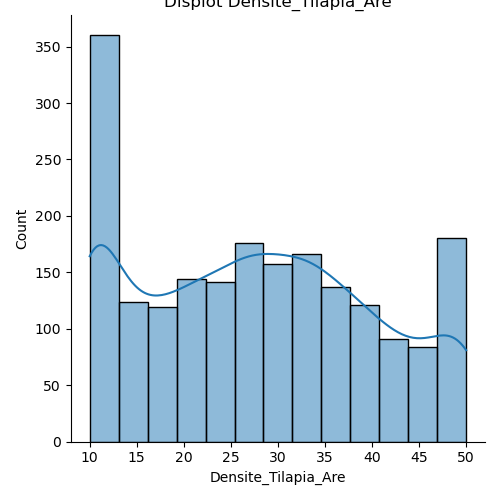
\includegraphics[width=0.4\textwidth]{Densite_tilapia/Displot Densite_Tilapia_Are.png}
\caption{Distribution de la variable Densite\_Tilapia\_Are}
\label{fig:displot_densite}
\textit{Source : Réalisation Personnelle}
\end{figure}


Les figures suivantes présentent, sous forme de violin plots, la relation entre la densité de tilapia et chacune des variables du dataset.

\begin{figure}[H]
\centering
\begin{minipage}{0.48\textwidth}
\centering
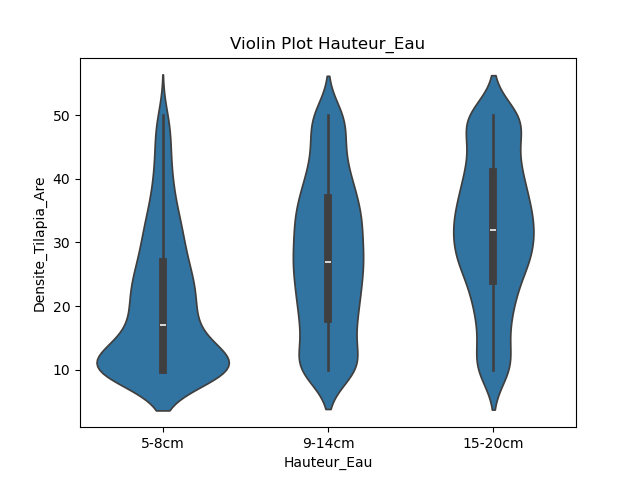
\includegraphics[width=\textwidth]{Densite_tilapia/ViolinPlot Hauteur_Eau.png}
\caption{Densité de tilapia selon la hauteur d'eau}
\label{fig:violin_hauteur_eau}
\textit{Source : Réalisation Personnelle}
\end{minipage}
\hfill
\begin{minipage}{0.48\textwidth}
\centering
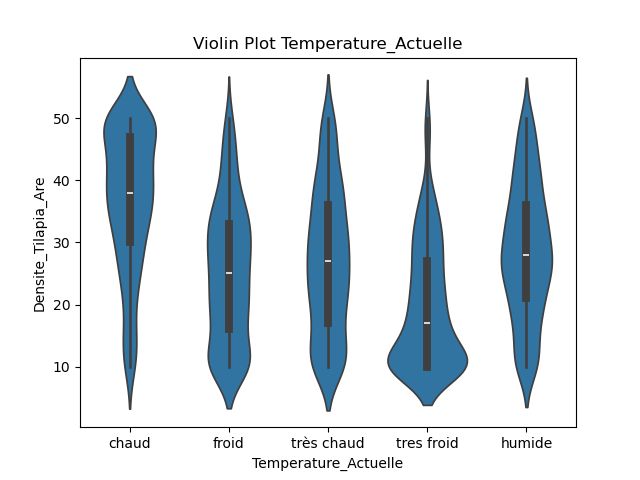
\includegraphics[width=\textwidth]{Densite_tilapia/Violin Plot Temperature_Actuelle.png}
\caption{Densité de tilapia selon la température actuelle}
\label{fig:violin_temperature}
\textit{Source : Réalisation Personnelle}
\end{minipage}
\end{figure}


La Figure~\ref{fig:violin_hauteur_eau} montre une tendance croissante claire : la médiane de densité passe d'environ 17 tilapias/are pour une hauteur d'eau de 5-8 cm, à environ 27 pour 9-14 cm, puis à environ 32 pour 15-20 cm. Sur le plan pratique, cela confirme une réalité bien connue des rizipisciculteurs : une lame d'eau trop faible limite l'espace de vie et de nage des poissons et les expose davantage aux variations de température, tandis qu'une hauteur d'eau suffisante offre un habitat plus stable et plus propice à leur croissance.

La Figure~\ref{fig:violin_temperature} révèle quant à elle que la catégorie « chaud » est associée à la médiane de densité la plus élevée (environ 38), tandis que la catégorie « tres froid » présente la médiane la plus basse (environ 17) et la distribution la plus resserrée vers les faibles valeurs, confirmant la sensibilité du tilapia aux températures basses.


\begin{figure}[H]
\centering
\begin{minipage}{0.48\textwidth}
\centering
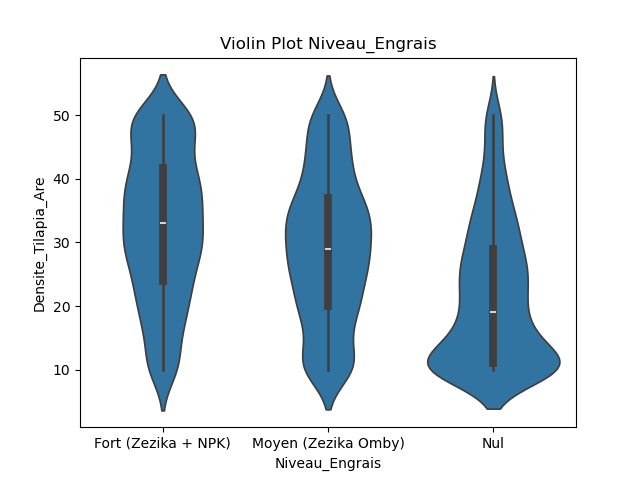
\includegraphics[width=\textwidth]{Densite_tilapia/Violin Plot Niveau_Engrais.png}
\caption{Densité de tilapia selon le niveau d'engrais}
\label{fig:violin_engrais}
\textit{Source : Réalisation Personnelle}
\end{minipage}
\hfill
\begin{minipage}{0.48\textwidth}
\centering
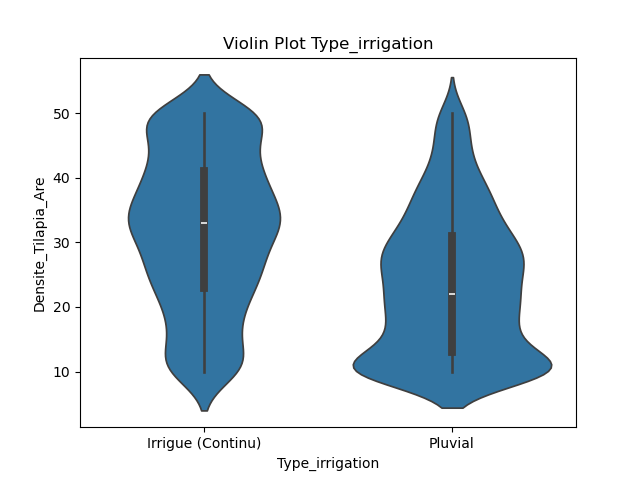
\includegraphics[width=\textwidth]{Densite_tilapia/Violin Plot Type_irrigation.png}
\caption{Densité de tilapia selon le type d'irrigation}
\label{fig:violin_irrigation}
\textit{Source : Réalisation Personnelle}
\end{minipage}
\end{figure}

La Figure~\ref{fig:violin_engrais} met en évidence une relation croissante entre le niveau de fertilisation et la densité de tilapia : la médiane passe d'environ 19 pour un niveau d'engrais nul, à environ 29 pour un niveau moyen, puis à environ 33 pour un niveau fort. cela s'explique par le fait que la fertilisation (notamment organique, comme le zezika traditionnellement utilisé à Madagascar) stimule le développement du plancton et des micro-organismes dont se nourrit le tilapia.

La Figure~\ref{fig:violin_irrigation} montre par ailleurs que les parcelles en irrigation continue présentent une médiane de densité nettement plus élevée (environ 33) que les parcelles en irrigation pluviale (environ 22), suggérant qu'un apport d'eau régulier favorise la croissance du cheptel piscicole.

\begin{figure}[H]
\centering
\begin{minipage}{0.48\textwidth}
\centering
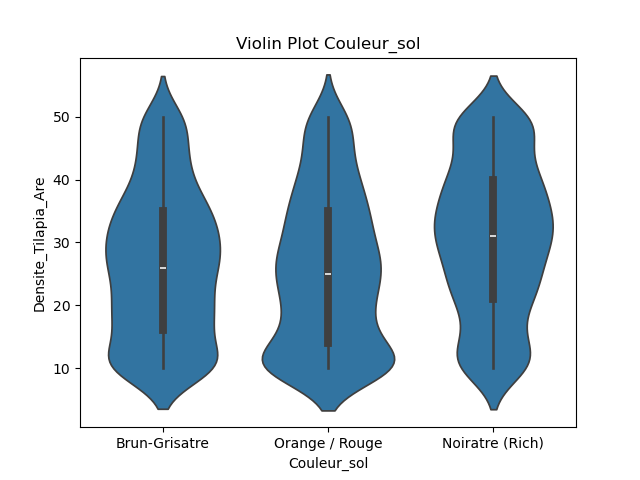
\includegraphics[width=\textwidth]{Densite_tilapia/Violin Plot Couleur_sol.png}
\caption{Densité de tilapia selon la couleur du sol}
\label{fig:violin_couleur}
\textit{Source : Réalisation Personnelle}
\end{minipage}
\hfill
\begin{minipage}{0.48\textwidth}
\centering
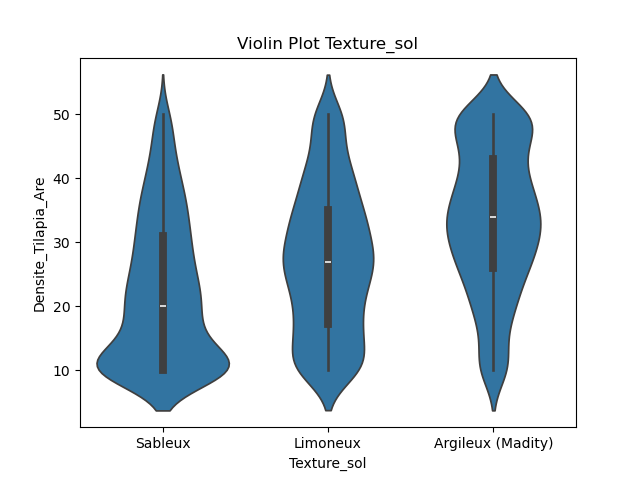
\includegraphics[width=\textwidth]{Densite_tilapia/Violin Plot Texture_sol.png}
\caption{Densité de tilapia selon la texture du sol}
\textit{Source : Réalisation Personnelle}

\label{fig:violin_texture}
\end{minipage}
\end{figure}

La Figure~\ref{fig:violin_couleur} montre des médianes assez proches entre les couleurs de sol « Brun-Grisâtre » et « Orange/Rouge » (autour de 25-26), tandis que le sol « Noirâtre (Rich) » présente une médiane légèrement supérieure (environ 31), cohérente avec sa richesse organique généralement plus élevée.

Enfin, la Figure~\ref{fig:violin_texture} révèle une tendance croissante selon la texture du sol : le sol sableux présente la médiane la plus basse (environ 20), le sol limoneux une médiane intermédiaire (environ 27), et le sol argileux la médiane la plus élevée (environ 34), ce dernier retenant probablement mieux l'eau et les nutriments nécessaires au développement du tilapia.\\

La Figure~\ref{fig:heatmap_densite} présente la matrice de corrélation entre les variables explicatives encodées et la variable cible \texttt{Densite\_Tilapia\_Are}.

\begin{figure}[H]
\centering
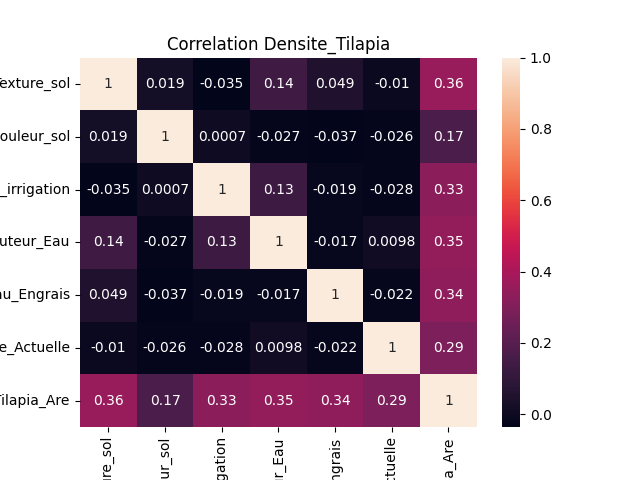
\includegraphics[width=0.55\textwidth]{Densite_tilapia/Heatmap Correlation.png}
\caption{Matrice de corrélation des variables du Module 1}
\label{fig:heatmap_densite}
\textit{Source : Réalisation Personnelle}
\end{figure}

On retrouve dans cette matrice les tendances déjà observées sur les violin plots précédents, désormais quantifiées. On remarque également que les variables explicatives sont globalement très peu corrélées entre elles , ce qui est plutôt favorable pour les modèles de régression linéaire, en limitant les risques de multicolinéarité. Cela confirme aussi que chacune de ces six variables apporte une information relativement indépendante et complémentaire à la prédiction de la densité de tilapia, justifiant leur intégration conjointe dans les modèles du Module 1.

\subsubsection{Qualité de l'eau}

Une analyse similaire a été menée sur le dataset de qualité de l'eau, en observant la distribution de chaque variable physico-chimique selon la classe de qualité (\texttt{label} = 0 pour mauvaise qualité, \texttt{label} = 1 pour bonne qualité), ainsi que l'équilibre général des classes.

\begin{figure}[H]
\centering
\begin{minipage}{0.48\textwidth}
\centering
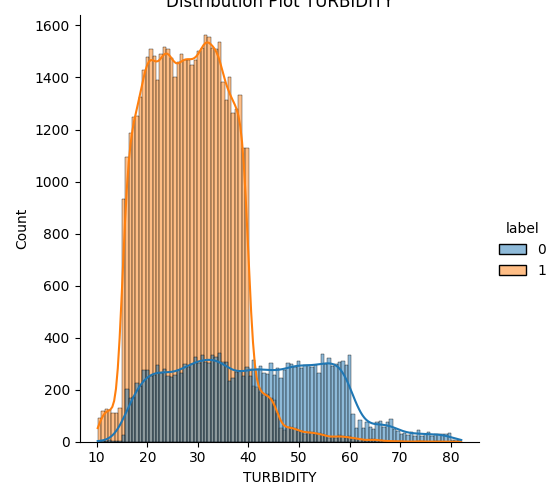
\includegraphics[width=\textwidth]{Qualite_eau/Distribution Plot TURBIDITY.png}
\caption{Distribution de la Turbidité selon la qualité de l'eau}
\textit{Source : Réalisation Personnelle}
\label{fig:dist_turbidity}
\end{minipage}
\hfill
\begin{minipage}{0.48\textwidth}
\centering
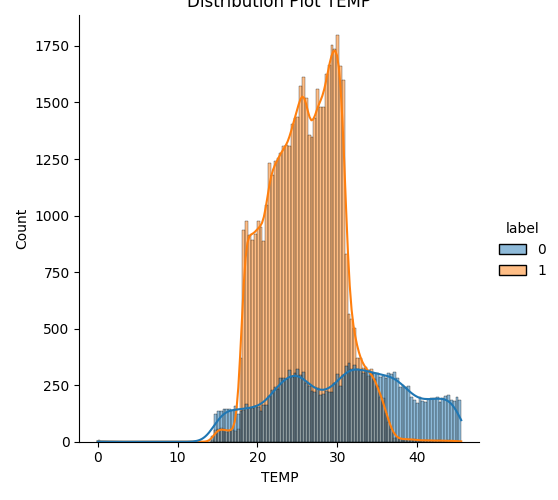
\includegraphics[width=\textwidth]{Qualite_eau/Distribution Plot TEMP.png}
\caption{Distribution de la Température selon la qualité de l'eau}
\textit{Source : Réalisation Personnelle}

\label{fig:dist_temp}
\end{minipage}
\end{figure}

La Figure~\ref{fig:dist_turbidity} montre une séparation assez nette entre les deux classes : les eaux de bonne qualité (label 1) se concentrent essentiellement entre 15 et 40 NTU, tandis que les eaux de mauvaise qualité (label 0) se répartissent surtout au-delà de 45 NTU, avec un pic marqué autour de 55-65. Concrètement, cela confirme qu'une eau trop trouble, chargée en particules en suspension, est un signal facilement identifiable de dégradation .

La Figure~\ref{fig:dist_temp} révèle une séparation encore plus marquée : les eaux de bonne qualité se situent majoritairement entre 15°C et 35°C, tandis que les eaux de mauvaise qualité se concentrent au-delà de 37°C. Cela correspond à une réalité bien connue : l'eau perd sa capacité à retenir l'oxygène nécessaire à la respiration des poissons, ce qui la rend rapidement dangereuse.

\begin{figure}[H]
\centering
\begin{minipage}{0.48\textwidth}
\centering
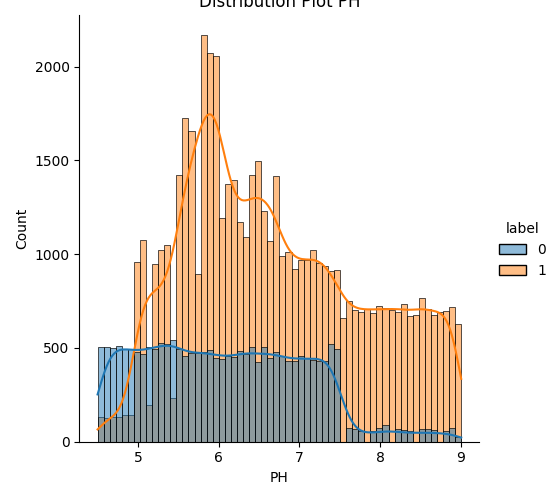
\includegraphics[width=\textwidth]{Qualite_eau/Distribution Plot PH.png}
\caption{Distribution du pH selon la qualité de l'eau}
\textit{Source : Réalisation Personnelle}
\label{fig:dist_ph}
\end{minipage}
\hfill
\begin{minipage}{0.48\textwidth}
\centering
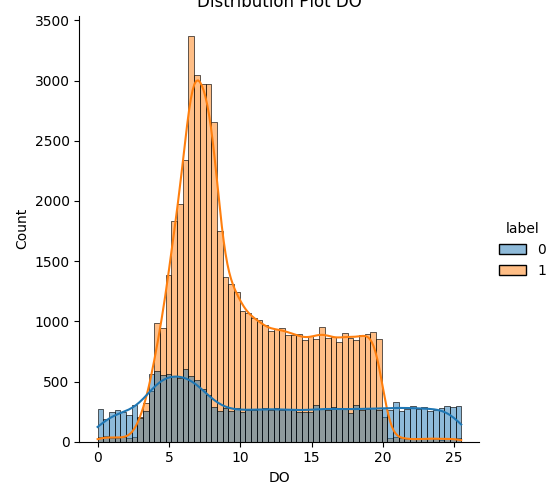
\includegraphics[width=\textwidth]{Qualite_eau/Distribution Plot DO.png}
\caption{Distribution de l'Oxygène Dissous selon la qualité de l'eau}
\textit{Source : Réalisation Personnelle}
\label{fig:dist_do}
\end{minipage}
\end{figure}

La Figure~\ref{fig:dist_ph} montre que les eaux de bonne qualité se concentrent surtout entre 5 et 7,5, avec un pic net autour de 6, tandis que les eaux de mauvaise qualité se répartissent plus largement au-delà de 7,5 et se prolongent jusqu'à 9. Un pH trop élevé (une eau trop basique) peut dégrader la santé des poissons.

La Figure~\ref{fig:dist_do} montre que les oxygènes dissous dans les eaux de bonne qualité se concentrent principalement entre 4 et 10 mg/L, avec un pic vers 6-7, tandis que les eaux de mauvaise qualité se répartissent sur une plage plus large, avec une proportion notable de valeurs très faibles (proches de 0) et très élevées (au-delà de 20). Un manque d'oxygène dissous est l'une des causes les plus fréquentes et les plus rapides de mortalité massive des poissons, souvent la nuit ou par forte chaleur.

La Figure~\ref{fig:heatmap_corr} présente la matrice de corrélation entre les différentes variables physico-chimiques et la variable cible.

\begin{figure}[H]
\centering

\includegraphics[width=0.55\textwidth]{Qualite_eau/Heatmap Correlation.png}
\caption{Matrice de corrélation entre les composants de l'eau}
\label{fig:heatmap_corr}
\textit{Source : Réalisation Personnelle}
\end{figure}

On observe que la variable \texttt{TURBIDITY} présente la corrélation la plus forte avec la qualité de l'eau (-0,48), ce qui confirme l'observation faite précédemment sur sa distribution : plus l'eau est trouble, plus elle a tendance à être classée en mauvaise qualité. La \texttt{TEMP} suit avec une corrélation de -0,35, cohérente avec la sensibilité du tilapia aux eaux trop chaudes. Le \texttt{PH} présente quant à lui une corrélation positive de 0,25, indiquant qu'un pH plus élevé est associé plus souvent à une bonne qualité dans ce dataset, tandis que le \texttt{DO} (oxygène dissous) affiche une corrélation plus faible (-0,13), ce qui peut sembler surprenant compte tenu de son importance biologique connue pour la survie des poissons, mais qui s'explique par le fait que son influence n'est pas linéaire : c'est surtout un déficit sévère en oxygène qui devient critique, plutôt qu'une simple variation continue de sa valeur. Cela justifie qu'un modèle non linéaire (comme la Random Forest ou XGBoost) puisse mieux capter cette relation qu'un simple coefficient de corrélation. On note enfin que les variables explicatives sont globalement peu corrélées entre elles (par exemple 0,094 entre PH et DO), ce qui limite les risques de multicolinéarité pour les modèles de classification développés dans le Module 2.

La Figure~\ref{fig:dist_qualite} présente enfin la répartition globale des deux classes dans le dataset.

\begin{figure}[H]
\centering
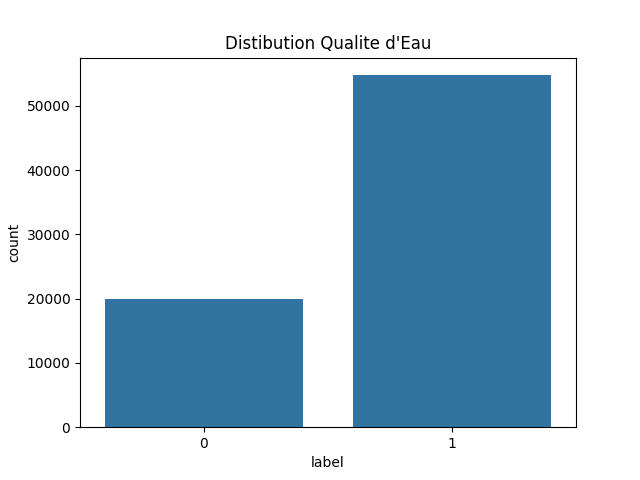
\includegraphics[width=0.4\textwidth]{Qualite_eau/Distibution Qualite d'Eau.png}
\caption{Répartition des classes de qualité de l'eau}
\textit{Source : Réalisation Personnelle}
\label{fig:dist_qualite}
\end{figure}

On observe un déséquilibre notable entre les deux classes : 54,746 observations sont étiquetées comme « bonne qualité » contre environ 20,012 comme « mauvaise qualité », soit une proportion d'environ 73~\% / 27~\%. Ce déséquilibre reflète une réalité plutôt rassurante sur le terrain : dans la majorité du temps, une parcelle correctement gérée conserve une eau de bonne qualité, les épisodes de dégradation restant l'exception plutôt que la norme. Cela confirme tout l'intérêt d'un système d'alerte : puisque les mauvais épisodes sont rares mais potentiellement lourds de conséquences (mortalité des poissons), il est essentiel de ne pas les manquer lorsqu'ils surviennent, ce qui devra être pris en compte dans le choix des métriques d'évaluation du modèle de classification (Module 2), afin de ne pas privilégier artificiellement la classe majoritaire au détriment de la détection des cas critiques.

\subsection{Prétraitement des données}

Avant l'entraînement des modèles, chaque dataset a fait l'objet d'étapes de nettoyage et de transformation spécifiques, adaptées à sa nature et à l'usage qui en est fait dans chacun des trois modules.

\subsubsection[Densité du tilapia]{Module 1 -- Densité du tilapia\\}
Le dataset contiens 75 doublons qui a été supprimé. Contrairement à une variable catégorielle sans relation d'ordre, chacune des variables catégorielles explicatives de ce dataset possède en réalité une progression logique entre ses modalités : la température va du plus froid au plus chaud, le niveau d'engrais du plus faible au plus fort, la texture du sol du plus filtrant (sableux) au plus retenant (argileux), la couleur du sol du plus clair au plus foncé (indicateur croissant de richesse organique), et le type d'irrigation d'un apport ponctuel (pluvial) à un apport continu. Un encodage one-hot ferait perdre cette information d'ordre, pourtant pertinente pour les modèles. Un encodage ordinal a donc été appliqué à la place, en associant à chaque modalité un entier croissant reflétant cette progression :


\begin{lstlisting}[language=Python]
temperature_encoder = {
    "TresFroid":0,
    "Froid":1,
    "Humide":2,
    "Chaud":3,
    "TresChaud":4,
}
niveaux_engrais_encoder = {
    "Nul":0,
    "Moyen":1,
    "Fort":2
}
texture_sol_encoder = {
    "Sableux":0,
    "Limoneux":1,
    "Argileux":2,
}
couleur_sol_encoder = {
    "Orange_Rouge":1,
    "Brun_Grisatre":2,
    "Noir":3
}
type_irrigation_encoder = {
    "Pluvial":0,
    "Continu":1
}
\end{lstlisting}

Cet encodage permet aux modèles, notamment ceux sensibles à la structure des variables comme la Régression Linéaire ou le SVR, d'exploiter directement la relation d'ordre entre les modalités, plutôt que de les traiter comme des catégories indépendantes sans lien entre elles.

\paragraph{Mise à l'échelle\\}
Conformément à la méthode de standardisation présentée en 3.2.4, les variables explicatives encodées du Module 1 (température, niveau d'engrais, texture et couleur du sol, type d'irrigation, hauteur d'eau) sont standardisées, afin de les ramener sur une échelle comparable avant l'entraînement des modèles sensibles à l'amplitude des variables, tels que la Régression Linéaire et le SVR.

\subsubsection[Classification de l'état actuel de l'eau]{Module 2 -- Classification de l'état actuel de l'eau\\}
Le dataset brut contenait 51 valeurs manquantes réparties sur ses 74 758 observations, soit une proportion négligeable (moins de 0,01 \% des cellules). Ces lignes incomplètes ont été supprimées plutôt qu'imputées. Aucun doublon n'a par ailleurs été détecté. La variable cible \texttt{label} étant déjà représentée sous forme binaire (0/1), aucun encodage supplémentaire n'est nécessaire pour celle-ci.

\paragraph{Mise à l'échelle\\}
Les variables physico-chimiques utilisées pour la classification (\texttt{PH}, \texttt{TEMP}, \texttt{DO}, \texttt{TURBIDITY}) possèdent des bornes physiques connues et fixes. Conformément à la méthode présentée en 3.2.4, une normalisation Min-Max (MinMaxScaler) est donc appliquée à ces variables, afin de les ramener dans un intervalle commun $[0,1]$ avant l'entraînement des modèles sensibles à l'échelle des données (Régression Logistique, SVC).

\subsubsection[Anticipation de la qualité de l'eau à H+1]{Module 3 -- Anticipation de la qualité de l'eau à H+1\\}
Le dataset brut, échantillonné toutes les 20 minutes, a été rééchantillonné à un pas de temps horaire, plus adapté à l'horizon de prédiction visé d'une heure, ce qui a réduit le dataset à 24 920 lignes, sans aucune valeur manquante après ce rééchantillonnage. Ce nouveau pas de temps régulier est indispensable pour appliquer la décomposition STL, qui nécessite une série temporelle à fréquence constante.

Une fois ce rééchantillonnage effectué, chaque variable physico-chimique est décomposée selon la méthode STL présentée en 3.2.2, en trois composantes : la tendance $T_t$, la saisonnalité $S_t$ et le résidu $R_t$. Ces trois composantes ne sont cependant pas traitées de la même façon dans la suite du pipeline.

La composante de tendance $T_t$, qui capture l'évolution de fond de la série, est celle qui alimente directement le modèle LSTM chargé de la prédiction à l'horizon d'une heure. La composante saisonnière $S_t$, quant à elle, correspond à un motif cyclique récurrent: plutôt que d'être réinjectée dans le modèle, elle est stockée séparément dans une base de données, et pourra être rajoutée à la prédiction de tendance issue du LSTM pour reconstituer une estimation complète de la valeur future.

Le résidu $R_t$, en revanche, est omis du pipeline de prédiction. Ce choix se justifie par le fait que la somme de la tendance et de la saisonnalité représente déjà environ 90 \% de la variance de la série originale, le résidu ne représentant donc qu'une faible part de l'information totale, correspondant essentiellement à du bruit de mesure difficilement prévisible par nature.

\paragraph{Mise à l'échelle\\}
Pour la composante de tendance $T_t$ utilisée dans le Module 3, une standardisation (Z-score) est appliquée plutôt qu'une normalisation Min-Max. En effet, contrairement aux valeurs brutes du Module 2, la tendance issue de la décomposition STL n'a pas de bornes fixes et connues à l'avance : elle peut évoluer au-delà des valeurs observées.

\paragraph{Feature Engineering\\}
Pour entraîner le modèle LSTM sur la composante de tendance $T_t$, celle-ci est restructurée selon une approche de fenêtre glissante : les trois derniers pas de temps de tendance ($T_{t-3}$, $T_{t-2}$, $T_{t-1}$) constituent les variables d'entrée (lags), tandis que la valeur de tendance à l'instant présent ($T_t$) constitue la variable cible à prédire. Cette formulation permet au modèle d'apprendre la relation entre l'évolution récente de la tendance et sa valeur suivante, ce qui correspond à l'usage classique des réseaux LSTM pour la prédiction de séries temporelles à un pas.

\subsection{Stratégie d'évaluation et découpage des données}

Une fois les données prétraitées, une stratégie d'évaluation adaptée à la nature de chaque tâche (régression, classification, prédiction temporelle) est nécessaire afin de mesurer honnêtement la capacité des modèles à généraliser, et de choisir des métriques pertinentes au regard des enjeux propres à chaque module.

\subsubsection[Densité du tilapia]{Module 1 -- Densité du tilapia\\}
\paragraph{Découpage des données\\}
Le dataset est séparé en un ensemble d'entraînement et un ensemble de test selon une proportion de 80 \%/20 \%. Le découpage est réalisé de façon aléatoire, la variable cible étant continue et ne présentant pas de déséquilibre de classes à préserver. L'ensemble de test n'intervient à aucun moment dans la phase d'entraînement ou d'optimisation des hyperparamètres, afin de fournir une estimation non biaisée de la performance finale des modèles.

\paragraph{Validation croisée et métriques\\}
Sur l'ensemble d'entraînement, une validation croisée à 3 folds est utilisée conjointement au GridSearch (voir 3.2.3) pour sélectionner les meilleurs hyperparamètres de chaque modèle. La performance finale de chaque modèle est ensuite mesurée sur l'ensemble de test à l'aide de quatre métriques adaptées à un problème de régression :
\begin{itemize}
    \item la RMSE (Root Mean Squared Error)
    \item la MAE (Mean Absolute Error)
    \item la MAPE (Mean Absolute Percentage Error)
    \item le $R^2$ (coefficient de détermination)
\end{itemize}
Ces quatre métriques sont calculées pour chacun des cinq modèles présentés en 3.2.1 (Régression Linéaire, SVM, Arbre de Décision, Random Forest, XGBoost), afin de les comparer sur une base commune.

\subsubsection[Classification de l'état actuel de l'eau]{Module 2 -- Classification de l'état actuel de l'eau\\}

\paragraph{Rééquilibrage des classes\\}
Le déséquilibre des classes observé en 4.3 risquant de biaiser l'apprentissage des modèles en faveur de la classe majoritaire, un rééquilibrage par sous-échantillonnage (downsampling) est appliqué : la classe majoritaire (« bonne qualité ») est réduite aléatoirement pour atteindre le même nombre d'observations que la classe minoritaire (« mauvaise qualité »), soit 20 012 lignes pour chacune des deux classes. Ce dataset équilibré est utilisé pour l'ensemble de la phase d'entraînement et d'évaluation du Module 2.

\paragraph{Découpage des données\\}
Le dataset équilibré est séparé en un ensemble d'entraînement et un ensemble de test selon une proportion de 70 \% / 30 \%. Le rééquilibrage préalable des classes rend un découpage stratifié moins critique qu'auparavant, celui-ci est néanmoins conservé par souci de rigueur méthodologique, afin de garantir une répartition strictement égale des deux classes dans les deux sous-ensembles.

\paragraph{Validation croisée et métriques\\}
Cinq métriques sont utilisées conjointement pour l'évaluation finale des modèles :
\begin{itemize}
    \item l'Accuracy, qui donne la proportion globale de prédictions correctes, désormais interprétable sans biais majeur grâce à l'équilibrage des classes ;
    \item la Precision, qui mesure, parmi les observations prédites comme « mauvaise qualité », la proportion réellement mauvaise ;
    \item le Recall (rappel), qui mesure, parmi les observations réellement de « mauvaise qualité », la proportion correctement détectée par le modèle -- la métrique la plus critique ici, puisqu'un cas de mauvaise qualité non détecté (faux négatif) expose directement les poissons à un risque, alors qu'une fausse alerte (faux positif) n'a qu'un coût opérationnel limité ;
    \item le F1-score, qui combine Precision et Recall en une seule valeur, utile pour comparer les modèles entre eux de façon synthétique;
\end{itemize}

\subsubsection[Anticipation de la qualité de l'eau à H+1]{Module 3 -- Anticipation de la qualité de l'eau à H+1\\}

\paragraph{Découpage des données\\}
Contrairement aux deux modules précédents, le découpage entraînement/test ne peut pas être aléatoire pour une série temporelle : il doit respecter l'ordre chronologique des observations, afin d'éviter que le modèle n'apprenne à partir d'informations futures qu'il ne posséderait pas en conditions réelles d'utilisation. L'ensemble d'entraînement correspond ainsi à la première partie chronologique de la composante de tendance $T_t$ restructurée en fenêtres glissantes, et l'ensemble de test à la période la plus récente.

\paragraph{Validation et métriques\\}
La performance du modèle LSTM est évaluée sur sa capacité à prédire $T_t$ à partir de $T_{t-3}$, $T_{t-2}$ et $T_{t-1}$, à l'aide des quatre mêmes métriques que pour le Module 1 : la RMSE, la MAE, la MAPE et le $R^2$, ce qui permet d'apprécier à la fois l'ampleur absolue et relative de l'erreur de prédiction sur la tendance.


\section{Mise en œuvre et évaluation des modules}

Ce chapitre constitue le cœur empirique de ce mémoire. Là où le Chapitre 3 a posé les fondements théoriques des modèles mobilisés et où le Chapitre 4 a préparé et structuré les données nécessaires, ce chapitre concrétise cette approche en mettant réellement en œuvre les trois modules du système rizipiscicole, puis en évaluant leurs performances respectives.

\subsection[Densité du tilapia]{Module 1 -- Densité du tilapia\\}

Pour le Module 1, dédié à l'estimation de la densité de tilapia à partir des caractéristiques du sol rizicole, les cinq modèles présentés en 3.2.1 (Régression Linéaire, Arbre de Décision, Random Forest, SVM, XGBoost) sont entraînés puis optimisés via la démarche de GridSearch présentée en 3.2.3. Pour chaque modèle, une grille d'hyperparamètres candidats est définie, et la meilleure combinaison est retenue par validation croisée. Les grilles testées pour chaque modèle sont détaillées dans les tableaux suivants.

\begin{longtable}{|p{5cm}|p{12cm}|}
\hline
\textbf{Hyperparamètre} & \textbf{Valeurs testées} \\
\hline

\texttt{fit\_intercept} & \texttt{True}, \texttt{False} \\
\hline
\caption{GridSearch-- Régression Linéaire} 
\end{longtable}
\begin{center}
\vspace{-0.85cm}
\end{center}
\begin{center}
\vspace{-0.85cm}
\textit{Source : Réalisation Personnelle}
\end{center}


\begin{longtable}{|p{5cm}|p{12cm}|}

\hline
\textbf{Hyperparamètre} & \textbf{Valeurs testées} \\
\hline
\texttt{criterion} & \texttt{squared\_error}, \texttt{friedman\_mse}, \texttt{absolute\_error}, \texttt{poisson} \\
\hline
\texttt{max\_depth} & \texttt{None}, 5, 10, 20 \\
\hline
\texttt{min\_samples\_split} & 2, 5, 10 \\
\hline
\texttt{min\_samples\_leaf} & 1, 2, 4 \\
\hline
\texttt{ccp\_alpha} & 0.0, 0.01, 0.1 \\
\hline
\texttt{max\_features} & \texttt{None}, \texttt{sqrt}, \texttt{log2} \\
\hline
\caption{GridSearch -- Arbre de Décision} \\
\end{longtable}
\begin{center}
\vspace{-0.85cm}
\textit{Source : Réalisation Personnelle}
\end{center}

\begin{longtable}{|p{5cm}|p{12cm}|}
\hline
\textbf{Hyperparamètre} & \textbf{Valeurs testées} \\
\hline
\texttt{n\_estimators} & 50, 100, 200 \\
\hline
\texttt{max\_depth} & \texttt{None}, 5, 10 \\
\hline
\texttt{min\_samples\_split} & 2, 5, 10 \\
\hline
\texttt{max\_features} & \texttt{sqrt}, \texttt{log2} \\
\hline
\caption{GridSearch-- Random Forest} \\
\end{longtable}
\begin{center}
\vspace{-0.85cm}
\textit{Source : Réalisation Personnelle}
\end{center}

\begin{longtable}{|p{5cm}|p{12cm}|}
\hline
\textbf{Hyperparamètre} & \textbf{Valeurs testées} \\
\hline
\texttt{C} & 0.1, 1, 10 \\
\hline
\texttt{kernel} & \texttt{linear}, \texttt{rbf}, \texttt{poly} \\
\hline
\texttt{gamma} & \texttt{scale}, \texttt{auto}, 0.1, 1 \\
\hline
\texttt{epsilon} & 0.1, 0.01, 0.001 \\
\hline
\caption{GridSearch -- SVM (SVR)} \\
\end{longtable}
\begin{center}
\vspace{-0.85cm}
\textit{Source : Réalisation Personnelle}
\end{center}

\begin{longtable}{|p{5cm}|p{12cm}|}
\hline
\textbf{Hyperparamètre} & \textbf{Valeurs testées} \\
\hline


\texttt{n\_estimators} & 50, 100, 200 \\
\hline
\texttt{learning\_rate} & 0.01, 0.1, 0.2 \\
\hline
\texttt{max\_depth} & 3, 5, 7, \texttt{None} \\
\hline
\texttt{min\_child\_weight} & 1, 3, 5 \\
\hline
\texttt{gamma} & 0, 0.1, 0.2 \\
\hline
\caption{GridSearch -- XGBoost} \\
\end{longtable}
\begin{center}
\vspace{-0.85cm}
\textit{Source : Réalisation Personnelle}
\end{center}

Ces cinq grilles sont explorées via \texttt{GridSearchCV}, combinée à une validation croisée, afin d'identifier pour chaque modèle la configuration d'hyperparamètres offrant la meilleure performance moyenne.

\subsubsection{Résultats de l'optimisation et évaluation}

\paragraph{Meilleurs hyperparamètres retenus\\}
Le tableau suivant présente, pour chacun des cinq modèles, la meilleure combinaison d'hyperparamètres identifiée par GridSearch, ainsi que le score moyen obtenu en validation croisée (correspondant au $R^2$).

\begin{longtable}{|p{3.5cm}|p{7cm}|p{1.8cm}|}

\hline
\textbf{Modèle} & \textbf{Meilleurs hyperparamètres} & \textbf{Score CV ($R^2$)} \\
\hline
Régression Linéaire & \texttt{fit\_intercept: True} & 0,5494 \\
\hline
Arbre de Décision & \texttt{ccp\_alpha: 0.01, criterion: friedman\_mse, max\_depth: None, max\_features: None, min\_samples\_leaf: 4, min\_samples\_split: 10} & 0,5759 \\
\hline
Random Forest & \texttt{max\_depth: 10, max\_features: sqrt, min\_samples\_split: 5, n\_estimators: 200} & 0,6542 \\
\hline
SVM (SVR) & \texttt{C: 10, epsilon: 0.1, gamma: scale, kernel: rbf} & 0,6518 \\
\hline
XGBoost & \texttt{gamma: 0, learning\_rate: 0.1, max\_depth: 3, min\_child\_weight: 5, n\_estimators: 100} & 0,6945 \\
\hline
\caption{Meilleurs hyperparamètres retenus par GridSearch -- Module 1} \\
\end{longtable}
\begin{center}
\vspace{-0.85cm}
\textit{Source : Réalisation Personnelle}
\end{center}


On observe que le score de validation croisée s'améliore progressivement à mesure que la complexité du modèle augmente.Cela suggère que la relation entre les caractéristiques du sol et la densité de tilapia n'est pas purement linéaire, et qu'elle bénéficie de modèles capables de capturer des interactions plus complexes entre les variables.

\paragraph{Performances sur l'ensemble de test\\}

La Figure~\ref{fig:eval_densite} présente la comparaison des cinq modèles selon les quatre métriques retenues (RMSE, MAE, MAPE, $R^2$).


\begin{figure}[H]
\centering
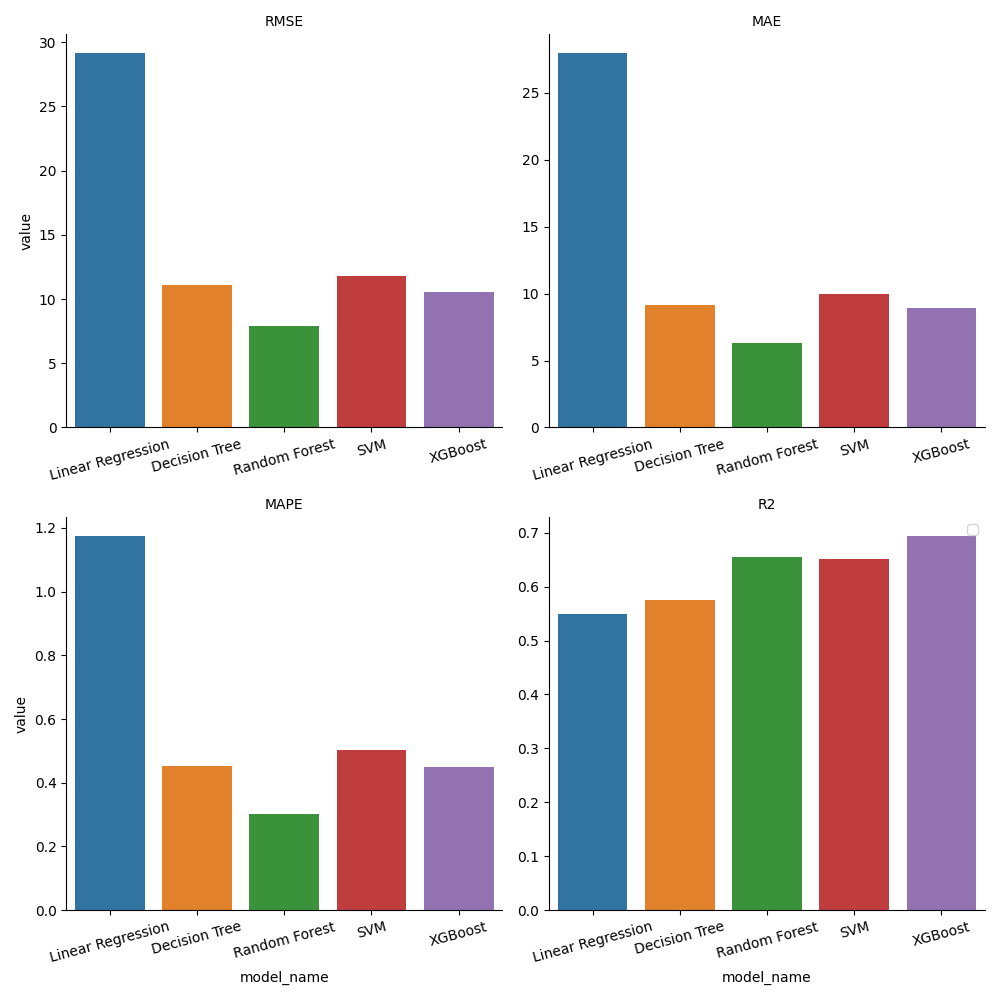
\includegraphics[width=0.65\textwidth]{Densite_tilapia/Evaluations Densite.png}
\caption{Comparaison des performances des modèles -- Module 1}
\label{fig:eval_densite}
\textit{Source : Réalisation Personnelle}
\end{figure}

La Régression Linéaire affiche les moins bonnes performances sur l'ensemble des quatre métriques, ce qui confirme les limites d'une relation purement linéaire pour ce problème.

Le SVM, malgré un score de validation croisée proche de celui de la Random Forest obtient une RMSE et une MAE nettement plus élevées sur l'ensemble de test , ce qui suggère une performance un peu moins stable ou une plus grande sensibilité aux valeurs extrêmes de ce modèle sur des données non vues.

La Random Forest et XGBoost se distinguent nettement des trois autres modèles, avec les RMSE les plus faibles et les $R^2$ les plus élevés . XGBoost obtient le meilleur $R^2$ global mais c'est la Random Forest qui présente la MAPE la plus faible, ce qui en fait, en termes relatifs, le modèle le plus précis pour estimer la densité de tilapia. Ces deux modèles, tous deux fondés sur des ensembles d'arbres de décision, apparaissent ainsi comme les plus adaptés pour ce module, la Random Forest et XGBoost pouvant être considérés comme équivalents en pratique, au profit de l'un ou l'autre selon que l'on privilégie l'erreur absolue relative (MAPE) ou la variance expliquée $R^2$.

\subsection[Classification de l'état actuel de l'eau]{Module 2 -- Classification de l'état actuel de l'eau\\}

Pour le Module 2, dédié à la classification de l'état actuel de la qualité de l'eau, les cinq modèles présentés en 3.2.1 (Régression Logistique, Arbre de Décision, Random Forest, SVM, XGBoost) sont entraînés puis optimisés via GridSearchCV. Les grilles d'hyperparamètres testées pour chaque modèle sont détaillées dans les tableaux suivants.

\begin{longtable}{|p{3.5cm}|p{9.5cm}|}
\hline
\textbf{Hyperparamètre} & \textbf{Valeurs testées} \\
\hline
\texttt{penalty} & \texttt{l1}, \texttt{l2} \\
\hline
\texttt{C} & 0.01, 0.1, 1 \\
\hline
\texttt{solver} & \texttt{saga} \\
\hline
\texttt{max\_iter} & 1000 \\
\hline
\caption{Grille d'hyperparamètres testés -- Régression Logistique} \\
\end{longtable}
\begin{center}
\vspace{-0.85cm}
\textit{Source : Réalisation Personnelle}
\end{center}

\begin{longtable}{|p{3.5cm}|p{9.5cm}|}
\hline
\textbf{Hyperparamètre} & \textbf{Valeurs testées} \\
\hline
\texttt{criterion} & \texttt{gini}, \texttt{entropy} \\
\hline
\texttt{max\_depth} & \texttt{None}, 10, 20 \\
\hline
\caption{Grille d'hyperparamètres testés -- Arbre de Décision} \\
\end{longtable}
\begin{center}
\vspace{-0.85cm}
\textit{Source : Réalisation Personnelle}
\end{center}

\begin{longtable}{|p{3.5cm}|p{9.5cm}|}
\hline
\textbf{Hyperparamètre} & \textbf{Valeurs testées} \\
\hline

\texttt{n\_estimators} & 20, 50, 100 \\
\hline
\texttt{max\_depth} & \texttt{None}, 10, 20 \\
\hline
\texttt{max\_features} & \texttt{sqrt}, \texttt{log2} \\
\hline
\caption{Grille d'hyperparamètres testés -- Random Forest} \\
\end{longtable}
\begin{center}
\vspace{-0.85cm}
\textit{Source : Réalisation Personnelle}
\end{center}

\begin{longtable}{|p{3.5cm}|p{9.5cm}|}
\hline
\textbf{Hyperparamètre} & \textbf{Valeurs testées} \\
\hline

\texttt{C} & 0.1, 1 \\
\hline
\texttt{gamma} & \texttt{scale}, \texttt{auto}, 0.01, 0.1 \\
\hline
\texttt{kernel} & \texttt{rbf}, \texttt{linear} \\
\hline
\caption{Grille d'hyperparamètres testés -- SVM (SVC)} \\
\end{longtable}
\begin{center}
\vspace{-0.85cm}
\textit{Source : Réalisation Personnelle}
\end{center}

\begin{longtable}{|p{3.5cm}|p{9.5cm}|}

\hline
\textbf{Hyperparamètre} & \textbf{Valeurs testées} \\
\hline

\texttt{n\_estimators} & 20, 50, 100 \\
\hline
\texttt{learning\_rate} & 0.01, 0.1, 0.2 \\
\hline
\texttt{max\_depth} & 3, 5, 7, \texttt{None} \\
\hline
\caption{Grille d'hyperparamètres testés -- XGBoost} \\
\end{longtable}
\begin{center}
\vspace{-0.85cm}
\textit{Source : Réalisation Personnelle}
\end{center}

Ces cinq grilles sont explorées via \texttt{GridSearchCV}, conformément à la stratégie d'évaluation présentée précédemment.


\subsubsection{Résultats de l'optimisation et évaluation}

\paragraph{Meilleurs hyperparamètres retenus\\}

\begin{longtable}{|p{3.5cm}|p{7cm}|p{1.8cm}|}
\hline
\textbf{Modèle} & \textbf{Meilleurs hyperparamètres} & \textbf{Score CV (Recall)} \\
\hline
Régression Logistique & \texttt{C: 0.1, max\_iter: 1000, penalty: l2, solver: saga} & 0,7716 \\
\hline
Arbre de Décision & \texttt{criterion: gini, max\_depth: 10} & 0,9069 \\
\hline
Random Forest & \texttt{max\_depth: 20, max\_features: sqrt, n\_estimators: 100} & 0,9243 \\
\hline
SVM (SVC) & \texttt{C: 1, gamma: scale, kernel: rbf} & 0,9035 \\
\hline
XGBoost & \texttt{learning\_rate: 0.1, max\_depth: 7, n\_estimators: 100} & 0,9237 \\
\hline
\caption{Meilleurs hyperparamètres retenus par GridSearch -- Module 2}
\end{longtable}
\begin{center}
\vspace{-0.85cm}
\textit{Source : Réalisation Personnelle}
\end{center}

On observe un écart très net entre la Régression Logistique, et l'ensemble des quatre autres modèles. Cet écart confirme que la frontière séparant une eau de bonne et de mauvaise qualité n'est pas linéaire : un modèle linéaire simple comme la Régression Logistique peine à capturer les interactions entre le pH, la température, l'oxygène dissous et la turbidité, contrairement aux modèles à base d'arbres et au SVM à noyau RBF, capables de modéliser des frontières de décision plus complexes.

\paragraph{Performances sur l'ensemble de test\\}
Le tableau suivant détaille les performances des cinq modèles selon les 4 métriques retenues (Accuracy, Precision, Recall, F1-score).

\begin{table}[H]
\centering
\begin{tabular}{|p{3.5cm}|p{1.9cm}|p{1.9cm}|p{1.9cm}|p{1.5cm}|p{1.9cm}|}
\hline
\textbf{Modèle} & \textbf{Accuracy} & \textbf{Precision} & \textbf{Recall} & \textbf{F1} \\
\hline
Régression Logistique & 0,7717 & 0,7731 & 0,7717 & 0,7713 \\
\hline
Arbre de Décision & 0,9151 & 0,9166 & 0,9151 & 0,9150  \\
\hline
Random Forest & 0,9253 & 0,9260 & 0,9253 & 0,9253  \\
\hline
SVM (SVC) & 0,9036 & 0,9060 & 0,9036 & 0,9034  \\
\hline
XGBoost & 0,9241 & 0,9250 & 0,9241 & 0,9240  \\
\hline
\end{tabular}
\caption{Performances des modèles sur l'ensemble de test -- Module 2}
\textit{Source : Réalisation Personnelle}
\end{table}


La Régression Logistique reste nettement en retrait sur l'ensemble des quatres métriques, avec un Recall de seulement 0,7717, ce qui signifierait, en conditions réelles, qu'environ un cas sur quatre de mauvaise qualité de l'eau passerait inaperçu -- un niveau de risque difficilement acceptable pour la protection du cheptel piscicole.

Les quatre autres modèles présentent des performances élevées et globalement proches. La Random Forest obtient le meilleur Recall (0,9253) ainsi que la meilleure Accuracy, Precision et F1-score, ce qui en fait le modèle le plus équilibré du Module 2. 

Au regard de la priorité donnée au Recall pour ce module, la Random Forest apparaît comme le choix le plus adapté, avec XGBoost comme alternative très proche.

\subsection[Anticipation de la qualité de l'eau à H+1]{Module 3 -- Anticipation de la qualité de l'eau à H+1\\}

Pour le Module 3, dédié à l'anticipation de la qualité de l'eau à l'horizon d'une heure, un modèle LSTM distinct est entraîné pour chacune des quatre variables physico-chimiques de l'eau (PH, TEMP, DO, TURBIDITY), sur la composante de tendance $T_t$ issue de la décomposition STL, standardisée selon la méthode présentée en 3.2.4. Chaque modèle utilise une architecture LSTM, entraînée à prédire la valeur de tendance à l'instant présent à partir des trois derniers pas de temps (voir 4.3).

\subsubsection{Résultats de l'évaluation}

\paragraph{Performances par variable\\}
Le tableau suivant résume les performances obtenues pour chacune des quatre variables, sur l'ensemble de test, selon les métriques retenues pour ce module (RMSE, MAE, MAPE, $R^2$).

\begin{longtable}{|p{2.3cm}|p{1.7cm}|p{1.7cm}|p{1.7cm}|p{1.7cm}|}

\hline
\textbf{Variable} & \textbf{RMSE} & \textbf{MAE} & \textbf{MAPE} & \textbf{$R^2$} \\
\hline

PH & 0,1617 & 0,1299 & 0,0188 & 0,9427 \\
\hline
TEMP & 0,6204 & 0,4677 & 0,0191 & 0,9480 \\
\hline
DO & 0,6228 & 0,4698 & 0,0414 & 0,9610 \\
\hline
TURBIDITY & 1,2058 & 0,9486 & 0,0334 & 0,9525 \\
\hline
\caption{Performances du modèle LSTM par variable -- Module 3} 
\end{longtable}
\begin{center}
\vspace{-0.85cm}
\textit{Source : Réalisation Personnelle}
\end{center}

Le PH présente les meilleures erreurs en valeur absolue (RMSE $\approx$ 0,16, MAE $\approx$ 0,13), ce qui est cohérent avec le fait que le pH de l'eau évolue généralement de façon lente et progressive.\\
L'Oxygène dissous obtient quant à elle le meilleur $R^2$ (0,9610), particulièrement rassurant compte tenu du rôle critique de ce paramètre dans la survie du tilapia malgré une MAPE légèrement plus élevée ($\approx$ 4,1 \%). \\
La Température affiche des résultats globalement similaires à ceux du pH en termes de $R^2$ ($\approx$ 0,95) et de MAPE ($\approx$ 1,9 \%), ce qui reste cohérent avec l'usage prévu du système : ce qui compte pour l'alerte préventive n'est pas la précision au dixième de degré près, mais la capacité du modèle à anticiper correctement la direction et l'ampleur générale de l'évolution de la température. \\
Enfin, la Turbidité affiche les valeurs de RMSE et de MAE les plus élevées en absolu parmi les quatre variables, ce qui s'explique par l'amplitude naturellement plus grande de cette variable observée précédemment (valeurs s'étendant globalement de 10 à plus de 80 NTU), plutôt que par une réelle difficulté supplémentaire du modèle à la prédire, comme le confirme son $R^2$ tout de même élevé (0,9525) et sa MAPE modérée ($\approx$ 3,3 \%).\\

Dans l'ensemble, ces résultats confirment la pertinence de l'approche combinant décomposition STL et LSTM pour anticiper l'évolution de la qualité de l'eau à l'horizon d'une heure, avec des performances homogènes et satisfaisantes sur les quatre variables physico-chimiques du système.



\section{Déploiement}

Afin de rendre les trois modules développés dans le chapitre précédent concrètement utilisables, une interface de démonstration a été mise en place sous la forme d'une application web simple. Elle permet de présenter de façon interactive le fonctionnement des trois modèles développés, en simulant leur usage à partir de valeurs saisies manuellement par l'utilisateur.

L'interface est organisée en trois onglets, correspondant chacun à l'un des trois modules du système.\\
Le premier onglet ,\textbf{Densité Tilapia} , l'utilisateur y renseigne les caractéristiques de sa parcelle (texture et couleur du sol, type d'irrigation, hauteur d'eau, niveau d'engrais, température actuelle) puis obtient une estimation de la densité de tilapia atteignable en cliquant sur « Prédire la densité ».

\begin{figure}[h]
\centering
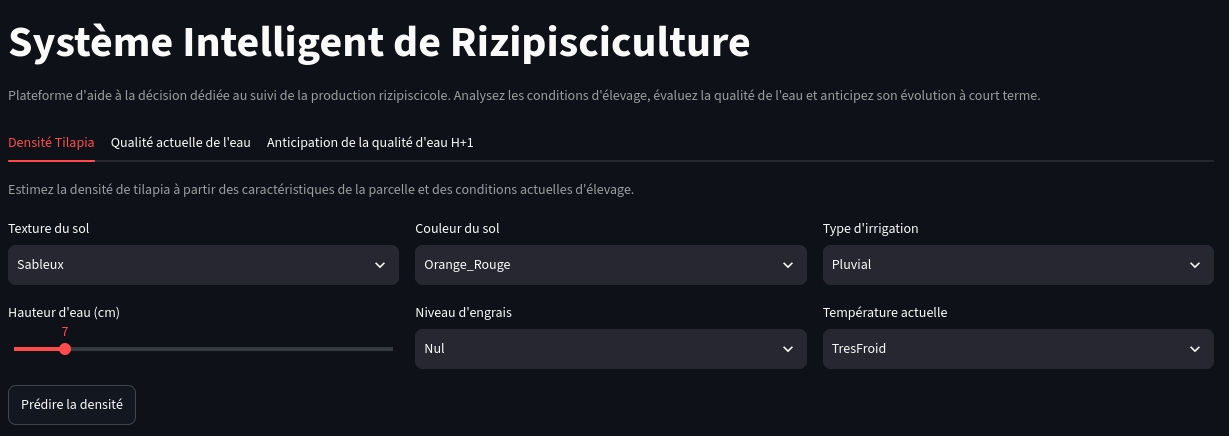
\includegraphics[width=0.85\textwidth]{Plateforme/Densite_Tilapia.jpg}
\caption{Interface du Module 1 -- Estimation de la densité de tilapia}
\textit{Source : Réalisation Personnelle}
\label{fig:interface_module1}
\end{figure}


Le deuxième onglet, \textbf{Qualité actuelle de l'eau}, l'utilisateur y saisit les quatre paramètres physico-chimiques mesurés à l'instant présent (PH, température, oxygène dissous, turbidité), et le bouton « Prédire la qualité » déclenche la classification de l'eau en bonne ou mauvaise qualité.

\begin{figure}[H]
\centering
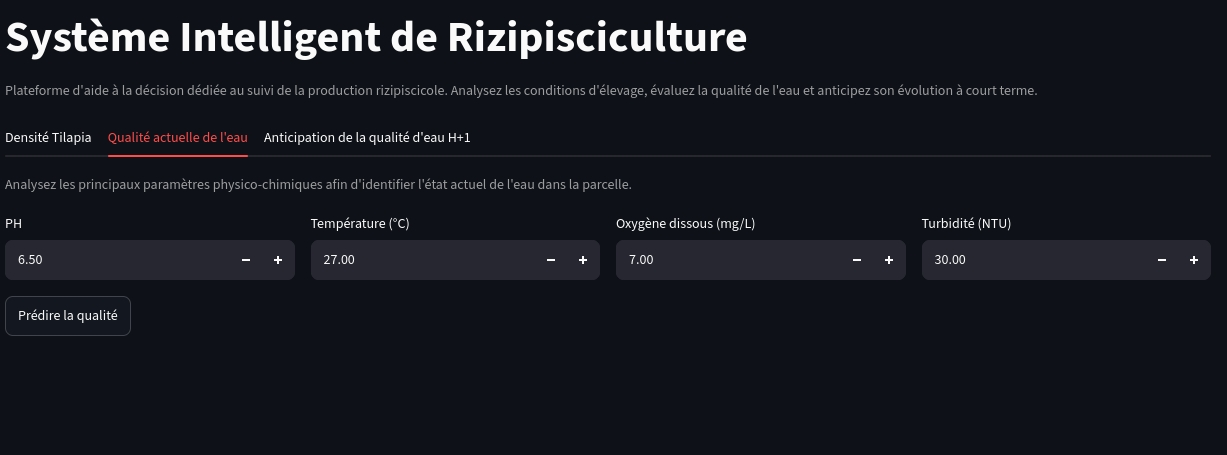
\includegraphics[width=0.85\textwidth]{Plateforme/Classification_Qualite_Eau.jpg}
\caption{Interface du Module 2 -- Classification de la qualité actuelle de l'eau}
\textit{Source : Réalisation Personnelle}
\label{fig:interface_module2}
\end{figure}

Le troisième onglet, « Anticipation de la qualité d'eau H+1 », l'utilisateur doit y renseigner les mêmes quatre paramètres physico-chimiques, mais pour trois instants successifs (deux heures avant, une heure avant, et l'heure actuelle), avant de cliquer sur « Anticiper » pour obtenir une estimation de l'état probable de l'eau une heure plus tard.

\begin{figure}[H]
\centering
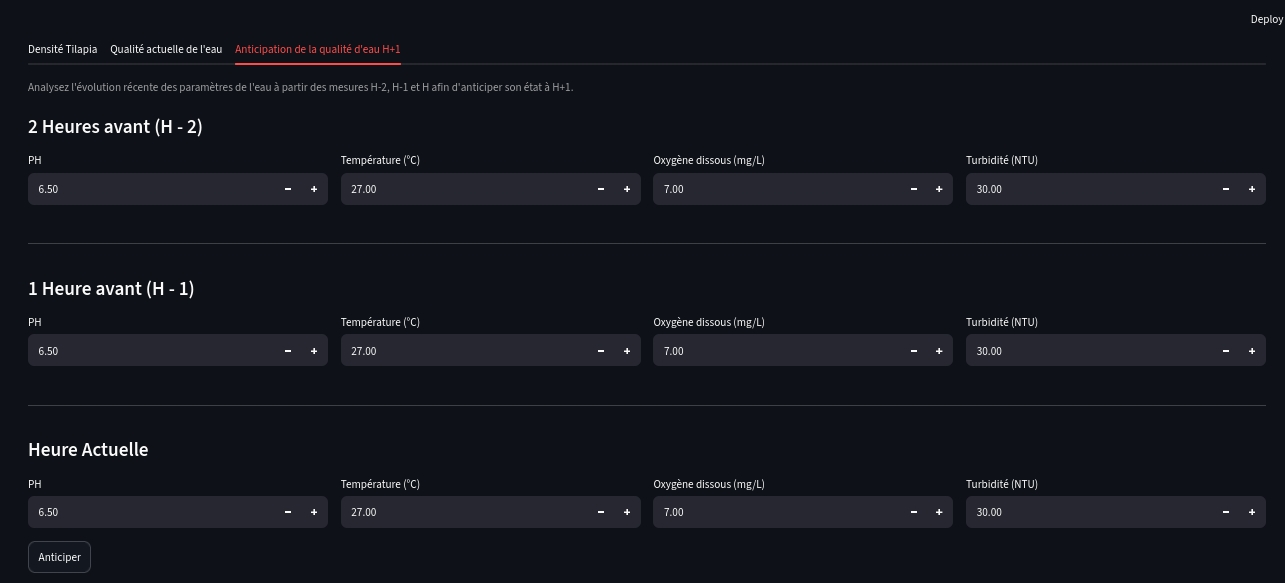
\includegraphics[width=0.85\textwidth]{Plateforme/Prediction_Qualite_Eau.jpg}
\caption{Interface du Module 3 -- Anticipation de la qualité de l'eau à H+1}
\textit{Source : Réalisation Personnelle}
\label{fig:interface_module3}
\end{figure}

\vspace*{\fill}
\newpage
\section*{\hfil \Large CONCLUSION \hfil}
\addcontentsline{toc}{section}{Conclusion}

La protection et l'optimisation de la production piscicole constituent un enjeu central pour le développement de la rizipisciculture, notamment dans un contexte comme celui de Madagascar, où cette pratique reste encore largement empirique malgré son fort potentiel. Ce mémoire a exploré cette problématique en combinant une analyse contextuelle du secteur rizipiscicole malgache, une exploration approfondie des données disponibles, et l'application de techniques avancées d'apprentissage automatique et de deep learning, afin de concevoir un Système Intelligent d'Analyse de Production Halieutique, composé de trois modules : l'estimation de la densité de tilapia, la classification de l'état actuel de la qualité de l'eau, et l'anticipation de son évolution à l'horizon d'une heure.

L'utilisation de modèles prédictifs plus avancés tels que la Random Forest, XGBoost, le SVM et les réseaux de neurones récurrents de type LSTM a permis de mieux capter des dynamiques sous-jacentes, avec des performances globalement satisfaisantes sur les trois modules développés. Ces résultats confirment qu'une analyse intelligente de la production halieutique, fondée sur les données, peut apporter une réponse concrète aux besoins de protection, d'anticipation et d'optimisation identifiés en introduction.

Ce travail présente néanmoins certaines limites qu'il convient de rappeler. Les données utilisées pour le module de densité de tilapia demeurent d'origine synthétique, faute d'accès à des mesures de terrain, et devront être confrontées à des données réelles. L'interface développée reste, elle aussi, un prototype de démonstration, reposant sur une saisie manuelle plutôt que sur une remontée automatique de données de capteurs.

Plusieurs perspectives peuvent ainsi être envisagées pour prolonger ce travail. Sur le plan des données, la priorité serait de valider les modèles à partir de mesures collectées directement sur des parcelles rizipiscicoles malgaches instrumentées, afin de confirmer la pertinence des résultats obtenus sur des données synthétiques ou issues d'autres contextes. Sur le plan technique, l'intégration de capteurs IoT permettrait une alimentation automatique et continue du système, réduisant la dépendance à une saisie manuelle et ouvrant la voie à des alertes réellement temps réel, rapprochant ainsi le système d'un véritable outil d'analyse intelligente de la production halieutique déployé au plus près du terrain.

En somme, ce projet offre une première contribution concrète à l'amélioration du suivi de la production rizipiscicole, à travers un système intelligent d'analyse de production halieutique encore perfectible mais fonctionnel, et ouvre la voie à des travaux futurs portant sur la validation des modèles à partir de données de terrain réelles, l'intégration de capteurs connectés, ainsi que le déploiement de l'interface développée sous une forme réellement accessible aux exploitants.



\vspace*{\fill}
\newpage
\pagenumbering{Roman}
\onehalfspacing
\renewcommand{\refname}{\hfil BIBLIOGRAPHIE \hfil}
\begin{thebibliography}{99}

\bibitem{iisd2023}
Institut International du Développement Durable (IISD).
\newline \textit{Fish for the future: From intensive to extensive aquaculture in Madagascar}. 2023. Disponible sur : \url{https://nbi.iisd.org/fr-fish-for-the-future-from-intensive-to-extensive-aquaculture-in-madagascar/}

\bibitem{apdra2023}
APDRA (Association Pisciculture et Développement Rural en Afrique).
\newline \textit{Rizipisciculture sur les hautes terres malagasy}. Résultats obtenus dans le cadre du Projet d'Aquaculture Durable à Madagascar (PADM), Janvier 2023.

\bibitem{minae}
Ministère de l'Agriculture et de la Souveraineté Alimentaire de Madagascar (MINAE).
\newline \textit{Agriculture à Madagascar : l'État déploie l'Infrastructure Publique Numérique Agricole pour soutenir les producteurs}. Disponible sur : \url{https://www.minae.gov.mg/agriculture-a-madagascar-letat-deploie-linfrastructure-publique-numerique-agricole-pour-soutenir-les-producteurs/}

\bibitem{lehnhoff2024}
\textit{Etho-acoustique et intelligence artificielle : application à la protection des cétacés}. Thèse de doctorat, 16 Septembre 2024. Disponible sur : \url{https://theses.hal.science/tel-04973790/}

\bibitem{nagpal2024}
\textit{Optimisation du traitement des eaux usées par intelligence artificielle}. 2024. DOI : \url{https://doi.org/10.2166/wst.2024.259}

\bibitem{abangan2023}
\textit{Intelligence artificielle pour la reconnaissance du comportement des poissons}. 23 Février 2023. DOI : \url{https://doi.org/10.3389/fmars.2023.1010761}

\bibitem{kilicarslan2024}
\textit{Détection de la fraîcheur du poisson par des approches d'intelligence artificielle}. 2024. DOI : \url{https://doi.org/10.24925/turjaf.v12i2.290-295.6670}

\bibitem{cao2021}
\textit{Prédiction de la teneur en oxygène dissous en aquaculture basée sur le regroupement et un ELM amélioré}. 4 Mars 2021. Disponible sur : \url{https://scispace.com/pdf/prediction-of-dissolved-oxygen-content-in-aquaculture-based4p8eytgpkn.pdf}

\bibitem{ozdemir2025}
\textit{Méthodes de Machine Learning pour évaluer l'impact des caractéristiques physico-chimiques de l'eau sur la consommation alimentaire dans les fermes piscicoles}. 14 Janvier 2025. DOI : \url{https://doi.org/10.15832/ankutbd.1470111}

\bibitem{cleveland1990}
\textit{STL: A Seasonal-Trend Decomposition Procedure Based on Loess}. Journal of Official Statistics, 6(1), 3--73.

\bibitem{cortesvapnik1995}
\textit{Support-Vector Networks}. Machine Learning, 20(3), 273--297. DOI : \url{https://doi.org/10.1007/BF00994018}

\bibitem{breiman2001}
\textit{Random Forests}. Machine Learning, 45(1), 5--32. DOI : \url{https://doi.org/10.1023/A:1010933404324}

\bibitem{hochreiter1997}
\textit{Long Short-Term Memory}. Neural Computation, 9(8), 1735--1780. DOI : \url{https://doi.org/10.1162/neco.1997.9.8.1735}

\bibitem{chenguestrin2016}
\textit{XGBoost: A Scalable Tree Boosting System}. Proceedings of the 22nd ACM SIGKDD International Conference on Knowledge Discovery and Data Mining. DOI : \url{https://doi.org/10.1145/2939672.2939785}

\bibitem{faotilapia}
FAO -- Fisheries and Aquaculture.
\newline \textit{Cultured Aquatic Species Information Programme -- Oreochromis niloticus}. Disponible sur : \url{https://www.fao.org/fishery/en/introsp/1756/en}

\bibitem{usgsturbidity}
United States Geological Survey (USGS).
\newline \textit{Turbidity and Water -- Water Science School}. Disponible sur : \url{https://www.usgs.gov/water-science-school/science/turbidity-and-water}

\end{thebibliography}
{\noindent\Large{\textbf{Cours Suivis:}}}
\begin{itemize}
\item{Docteur ANDRIAMANJAKA Ramasondrano : 
	\begin{itemize}
		\item{Python pour la Data Science}
		\item{Apprentissage Supervisé}
		\item{Apprentissage Non Supervisé}
	\end{itemize}
}
\vspace{0.5cm}
\item{Docteur RANDRIAMAMONJY Liantsoa Joharinirina : 
	\begin{itemize}
		\item{Introduction au Deep Learning}
	\end{itemize}
}
\vspace{0.5cm}
\item{Docteur RANDRIANIRINA Jean Marc Fabien :
	\begin{itemize}
		\item{Analyse de donnée}
	\end{itemize}
}
\end{itemize}

\newpage

\renewcommand{\refname}{\hfil WEBOGRPAHIE \hfil}
\begin{thebibliography}{99}

\bibitem{kagglefishlife}
Muzamil Aslam.
\newline \textit{Fish Life Prediction Dataset}. Kaggle. Disponible sur : \url{https://www.kaggle.com/datasets/muzamilaslam/fish-life-prediction/data}

\bibitem{scikitlearn}
\textit{Scikit-learn: Machine Learning in Python}. Disponible sur : \url{https://scikit-learn.org/stable/documentation.html}

\bibitem{xgboostdoc}
\textit{XGBoost Documentation}. Disponible sur : \url{https://xgboost.readthedocs.io/}

\bibitem{tensorflowdoc}
\textit{TensorFlow Documentation}. Disponible sur : \url{https://www.tensorflow.org/guide}

\bibitem{kerasdoc}
\textit{Keras Documentation}. Disponible sur : \url{https://keras.io/}

\bibitem{statsmodelsdoc}
\textit{Statsmodels Documentation -- STL Decomposition}. Disponible sur : \url{https://www.statsmodels.org/stable/generated/statsmodels.tsa.seasonal.STL.html}

\bibitem{fpp3}
\textit{Forecasting: Principles and Practice (3rd edition)}. Disponible sur : \url{https://otexts.com/fpp3/}

\bibitem{pandasdoc}
\textit{Pandas Documentation}. Disponible sur : \url{https://pandas.pydata.org/docs/}

\bibitem{numpydoc}
\textit{NumPy Documentation}. Disponible sur : \url{https://numpy.org/doc/}

\bibitem{seaborndoc}
\textit{Seaborn Documentation}. Disponible sur : \url{https://seaborn.pydata.org/}

\bibitem{matplotlibdoc}
\textit{Matplotlib Documentation}. Disponible sur : \url{https://matplotlib.org/stable/index.html}

\bibitem{imblearndoc}
\textit{Imbalanced-learn Documentation -- Under-sampling}. Disponible sur : \url{https://imbalanced-learn.org/stable/under_sampling.html}

\bibitem{streamlitdoc}
\textit{Streamlit Documentation}. Disponible sur : \url{https://docs.streamlit.io/}

\end{thebibliography}
\vspace*{\fill}
\newpage
\singlespacing 
\section*{\hfil ANNEXES \hfill}
\addcontentsline{toc}{section}{ANNEXES}

\subsection*{Extraits de code -- Classes de prédiction du système}

\subsubsection*{Module 1 -- Densité de tilapia (\texttt{DensiteTilapia.py})}

Cette classe charge le modèle XGBoost retenu pour l'estimation de la densité de tilapia , ainsi que les dictionnaires d'encodage ordinal, nécessaires pour convertir les variables catégorielles saisies par l'utilisateur en valeurs numériques avant de les transmettre au modèle.
\begin{lstlisting}[style=pythonstyle,language=Python, caption={Classe DensiteTilapia -- Module 1}, basicstyle=\ttfamily\scriptsize]
import pickle
import os

class DensiteTilapia:
    # Variables d'entree attendues :
    # Texture_sol, Couleur_sol, Type_irrigation, Hauteur_Eau, Niveau_Engrais, Temperature_Actuelle
    def __init__(self):
        # Dictionnaires d'encodage ordinal, refletant la progression logique de chaque
        self.temperature_encoder = {
            "TresFroid": 0,
            "Froid": 1,
            "Humide": 2,
            "Chaud": 3,
            "TresChaud": 4,
        }
        self.niveaux_engrais_encoder = {
            "Nul": 0,
            "Moyen": 1,
            "Fort": 2
        }
        self.texture_sol_encoder = {
            "Sableux": 0,
            "Limoneux": 1,
            "Argileux": 2,
        }
        self.couleur_sol_encoder = {
            "Orange_Rouge": 1,
            "Brun_Grisatre": 2,
            "Noir": 3
        }
        self.type_irrigation_encoder = {
            "Pluvial": 0,
            "Continu": 1
        }

        print("Chargement Du modele de Prediction de Densite Tilapia ... ")

        # Chargement du modele XGBoost retenu apres optimisation par GridSearch
        with open(os.path.join("models", "densite_tilapia_xgboost.pkl"), "rb") as file:
            model = pickle.load(file)

        print("Chargement avec Succes ... ")
        self.model = model

    def predict(self, texture, couleur, type_irrigation, hauteur_eau, engrais, temperature):
        # Encodage ordinal des variables categorielles saisies par l'utilisateur
        encoded_features = [
            self.texture_sol_encoder[texture],
            self.couleur_sol_encoder[couleur],
            self.type_irrigation_encoder[type_irrigation],
            hauteur_eau,
            self.niveaux_engrais_encoder[engrais],
            self.temperature_encoder[temperature]
        ]

        # Prediction de la densite de tilapia (nombre d'individus par are)
        prediction = self.model.predict([encoded_features])
        return prediction[0]
\end{lstlisting}


\subsubsection*{Module 2 -- Classification de la qualité de l'eau (\texttt{QualiteEau.py})}

Cette classe charge le modèle XGBoost retenu à l'issue de l'optimisation par GridSearch, et l'utilise pour classer l'état de l'eau en bonne ou mauvaise qualité à partir des quatre paramètres physico-chimiques mesurés à l'instant présent.

\begin{lstlisting}[style=pythonstyle,language=Python, caption={Classe QualiteEau -- Module 2},basicstyle=\ttfamily\scriptsize]
import pickle
import os

class QualiteEau:
    # Donnee d'entree attendue : PH, TEMP, DO, TURBIDITY (mesures a l'instant present)
    def __init__(self):
        print("Chargement Du modele de Classification d'Eau ... ")

        # Chargement du modele XGBoost retenu apres optimisation par GridSearch
        with open(os.path.join("models", "qualite_eau_xgboost.pkl"), "rb") as file:
            model = pickle.load(file)

        print("Chargement avec Succes ... ")
        self.model = model

    def predict(self, ph, temp, do, turbidity):
        # Mise en forme des 4 parametres en une seule observation
        input_data = [[ph, temp, do, turbidity]]

        # Classification : 0 = mauvaise qualite, 1 = bonne qualite
        prediction = self.model.predict(input_data)
        return prediction[0]
\end{lstlisting}

\subsubsection*{Module 3 -- Anticipation de la qualité de l'eau (\texttt{PredictionEau.py})}

Cette classe charge les quatre modèles LSTM entraînés (un par variable physico-chimique : PH, TEMP, DO, TURBIDITY), ainsi que les objets de standardisation (scalers) associés, nécessaires pour ramener les données d'entrée à l'échelle utilisée lors de l'entraînement, avant de les fournir au modèle.

\begin{lstlisting}[style=pythonstyle, caption={Classe PredictionEau -- Module 3},,basicstyle=\ttfamily\scriptsize]
import pickle
import os
import numpy as np
from statsmodels.tsa.seasonal import STL
from db import get_saisonnalite

class PredictionEau:
    # Liste des quatre variables physico-chimiques prises en charge par le module
    VARS = ["PH", "TEMP", "DO", "TURBIDITY"]

    # Correspondance entre le nom de la variable et le nom de sa colonne de saisonnalite en base
    COL_MAP = {"PH": "s_ph", "TEMP": "s_temp", "DO": "s_do", "TURBIDITY": "s_turbidity"}

    # Donnee d'entree attendue : PH, TEMP, DO, TURBIDITY (aux 3 derniers pas de temps)
    def __init__(self):
        print("Chargement Du modele de Prediction d'Eau ... ")
        self.model = {}
        self.scaler = {}

        # Chargement du modele LSTM entraine sur la composante de tendance du PH
        with open(os.path.join("models", "Timeseries_DL_PH_trend_LSTM_64.pkl"), "rb") as file:
            model = pickle.load(file)
        self.model["PH"] = model

        # Chargement du modele LSTM entraine sur la composante de tendance de la temperature
        with open(os.path.join("models", "Timeseries_DL_TEMP_trend_LSTM_64.pkl"), "rb") as file:
            model = pickle.load(file)
        self.model["TEMP"] = model

        # Chargement du modele LSTM entraine sur la composante de tendance de l'oxygene dissous
        with open(os.path.join("models", "Timeseries_DL_DO_trend_LSTM_64.pkl"), "rb") as file:
            model = pickle.load(file)
        self.model["DO"] = model

        # Chargement du modele LSTM entraine sur la composante de tendance de la turbidite
        with open(os.path.join("models", "Timeseries_DL_TURBIDITY_trend_LSTM_64.pkl"), "rb") as file:
            model = pickle.load(file)
        self.model["TURBIDITY"] = model

        # Chargement du scaler (standardisation) associe a chaque variable, utilise pour
        # ramener les donnees d'entree sur la meme echelle que celle vue a l'entrainement
        with open(os.path.join("models", "PH_trend_scaler.pkl"), "rb") as file:
            scaler = pickle.load(file)
        self.scaler["PH"] = scaler

        with open(os.path.join("models", "TEMP_trend_scaler.pkl"), "rb") as file:
            scaler = pickle.load(file)
        self.scaler["TEMP"] = scaler

        with open(os.path.join("models", "DO_trend_scaler.pkl"), "rb") as file:
            scaler = pickle.load(file)
        self.scaler["DO"] = scaler

        with open(os.path.join("models", "TURBIDITY_trend_scaler.pkl"), "rb") as file:
            scaler = pickle.load(file)
        self.scaler["TURBIDITY"] = scaler

        print("Chargement avec Succes ... ")

    def predict(self, ph_list, temp_list, do_list, turbidity_list, hour_of_year_target):
        """
        ph_list, temp_list, etc. : liste de 3 valeurs (lags H-2, H-1, H)
        hour_of_year_target : index de l'heure H+1 a predire (1 a ~8800 sur l'annee)
        """
        inputs = {
            "PH": ph_list,
            "TEMP": temp_list,
            "DO": do_list,
            "TURBIDITY": turbidity_list
        }

        predictions_finales = {}

        for var in self.VARS:
            # 1. Extraction de la tendance via la decomposition STL
            res = STL(inputs[var], period=3, robust=True).fit()
            tendance = res.trend

            # 2. Reshape en (3, 1) pour appliquer le scaler sur les donnees brutes
            tendance_3_1 = np.array(tendance).reshape(3, 1)
            tendance_scaled = self.scaler[var].transform(tendance_3_1)

            # 3. Reshape en (1, 3, 1) [Samples, Timesteps, Features] pour l'entree du modele LSTM
            input_modele = tendance_scaled.reshape(1, 3, 1)

            # 4. Prediction de la tendance standardisee pour l'instant H+1
            pred_trend_scaled = self.model[var].predict(input_modele)

            # 5. Inversion de la standardisation pour retrouver la vraie valeur de la tendance
            pred_trend = self.scaler[var].inverse_transform(pred_trend_scaled.reshape(1, 1))[0][0]

            # 6. Recuperation de la saisonnalite stockee en base pour l'heure ciblee
            nom_composant_sql = self.COL_MAP[var]
            saisonnalite_sql = get_saisonnalite(nom_composant_sql, hour_of_year_target)

            # 7. Reconstruction du signal final (tendance predite + saisonnalite)
            predictions_finales[var] = pred_trend + saisonnalite_sql

        return predictions_finales
\end{lstlisting}

\vspace*{\fill}
\newpage
\vspace*{\fill}
\begin{center}

	{\bfseries\large FICHE DE RENSEIGNEMENTS}
\end{center}

\vspace*{1cm}
\begin{flushleft}
    \begin{tabular}{@{}ll}
        \textbf{Nom :} & ANDRIAMIHAJAMANANA\\[0.3cm]
        \textbf{Prénom :} & Anjara \\[0.3cm]
        \textbf{Adresse :} & Lot 56 Bis Ankadiaivo Alasora \\[0.3cm]
        \textbf{Téléphone :} & 0381502522 \\[0.3cm]
        \textbf{Email :} & andriamihajamananaanjara@gmail.com
    \end{tabular}
    
    \vspace*{1.5cm}
    
    \noindent \textbf{Titre : SYSTÈME INTELLIGENT D'ANALYSE DES PRODUCTIONS HALIEUTIQUES}
    
    \vspace*{1.5cm}
    
    \begin{longtable}{p{4.5cm}p{13cm}}
        \textbf{Nombre de pages :} & 57 \\[0.3cm]
        \textbf{Mots clés :} & productions halieutiques, rizipisciculture, qualité de l'eau, machine learning, séries temporelles, LSTM, aide à la décision.\\[0.3cm]
        \textbf{Encadreur :} & Docteur RAMASONDRANO Andriamanjaka\\[0.3cm]
        \textbf{Grade :} & Docteur \\[0.3cm]
        \textbf{Téléphone :} & 0347289632 \\[0.3cm]
        \textbf{Email :} & ramasondranoandriamanjaka@gmail.com
    \end{longtable}
\end{flushleft}
\vspace*{\fill}
\end{document}

